\documentclass[runningheads]{llncs}
\usepackage[T1]{fontenc}
\usepackage{graphicx}
\usepackage{amsmath}
\usepackage{amssymb}
\usepackage{enumitem}
\usepackage{multirow}
\usepackage{tabularx}
\usepackage{ragged2e}
\usepackage{booktabs} 
\usepackage{subcaption}
\usepackage[misc]{ifsym}
\newcommand{\corr}{(\Letter)}
% N.B.: do not change anything above this line. If you require additional packages, please load them directly after this line.
\usepackage{mwe}
% N.B.: you may delete the preceding line. It is used to display an example image in this template.

\begin{document}

\title{Understanding Implications of Dataset Choice for Feature Effect Estimation:
    A Simulation-Based Investigation through Error Decomposition}

\titlerunning{Understanding Implications of Dataset Choice for Feature Effect Estimation}
% If the full title of your paper is short enough to also fit in the running head, you can omit the abbreviated paper title here. You can check as follows: if you comment out the \titlerunning line, something will appear in the header of all odd-numbered pages of your PDF from page 3 onward. This something is either the full title (in which case all is well), or the error message "Title Suppressed Due to Excessive Length". If this error message appears, you're going to want to provide an abbreviated title within the \titlerunning command, because if you won't do it, Springer will do it for you.

%N.B.: Author information (both in the \author{} and \authorrunning{} command) should only be present in the Camera-Ready Version of your paper. The version that you initially submit for review, ought to be double-blind. So, when initially submitting your paper, use:
%\author{Author information scrubbed for double-blind reviewing}
\author{Timo Heiß\inst{1}}
% You may leave out the orcidID information, if you want to.
% Use \corr to indicate the corresponding author. Note the spacing around the \corr command. Only one author can be the corresponding author.

%N.B.: comment out the \authorrunning{} command for the double-blind version of your paper submitted for review. Later, if your paper is accepted, use the command for the Camera-Ready Version.
\authorrunning{Timo Heiß}
% First names are abbreviated in the running head.
% If there is one author, write 'A.L. Benjamin'.
% If there are two authors, write 'A.L. Benjamin and C.C. Broadus Jr.'
% If there are more than two authors, '[...] et al.' is used.

\institute{Department of Statistics, LMU Munich, Ludwigstr. 33, 80539 Munich, Germany \email{t.heiss@campus.lmu.de}}

\maketitle              % typeset the header of the contribution

\begin{abstract}
    The abstract should briefly summarize the contents of the paper in
    150--250 words.

    \keywords{Explainable AI  \and Feature effects \and Partial dependence plot \and Accumulated local effects}
\end{abstract}

\section{Introduction}
Most Machine Learning (ML) models can be considered black boxes --- opaque
systems that intrinsically do not allow insight into their internal reasoning,
making it often impossible to explain their decisions. However, this can be
problematic in many critical domains and applications, such as the healthcare,
legal, or finance sectors, where decisions must be transparent and
accountable~\cite{adadi_peeking_2018}.

Interpretability in ML is crucial to enhance
trust~\cite{ribeiro_why_2016,teach_analysis_1981}, address potential
biases~\cite{guidotti_survey_2019}, fairness and ethical concerns
~\cite{lipton_mythos_2018}, and ensure compliance with regulations such as the
EU's General Data Protection Regulation (GDPR)~\cite{gdpr2016} and AI
Act~\cite{euaia2024}. To address these challenges, the field of Explainable AI
/ Interpretable ML has emerged~\cite{adadi_peeking_2018}. In the last years, a
wide variety of methods has been developed, including model-specific and
model-agnostic approaches ranging from local feature attributions to global
feature importances and effects\footnote{For an overview of Explainable AI
    methods, see
    e.g.~\cite{adadi_peeking_2018,kamath_introduction_2021,molnar_interpretable_2022}.}.

Due to the severity of many applications, it is crucial to utilize these
explainability methods correctly to avoid misleading or incorrect conclusions.
In general, there are many pitfalls to be aware of~\cite{molnar_general_2022},
including whether to compute explanations in-sample, i.e.\ on training data, or
out-of-sample, which we refer to as validation data in the following. Existing
works have studied the implications of this choice for many methods, including
studies on \textit{Permutation Feature Importance (PFI) } (e.g.,
in~\cite{molnar_general_2022}), \textit{Mean Decrease in Impurity (MDI)} of
Random Forests~\cite{loecher_debiasing_2022}, or \textit{SHAP}
values~\cite{loecher_debiasing_2024}.

However, to the best of our knowledge, there exist no such systematic studies
for feature effect methods like \textit{Partial Dependence Plots
    (PDP)}~\cite{friedman_greedy_2001} and \textit{Accumulated Local Effects
    (ALE)}~\cite{apley_visualizing_2020}. Current literature
(e.g.,~\cite{apley_visualizing_2020,friedman_greedy_2001,molnar_interpretable_2022})
predominantly uses training data without explicit justification, while
practitioners also advocate for using unseen validation data (for details, see
\textsc{Section~\ref{sec:related-works}}). Factors that may influence this
choice include potential biases arising from overfitting, the dataset size, and
computational constraints. Although PDP and ALE are not based on generalization
error like PFI, it is not studied if and how they are affected by overfitting.
In addition, larger datasets may improve the feature effect estimates, but also
increase computation times.\\

\noindent In this paper, we aim to answer the largely unaddressed, fundamental
methodological question of whether to use training or validation data to
compute feature effects. We perform an empirical simulation study, estimating
PDP and ALE on training data, validation data, and in a cross-validated manner
for different models and dataset. We decompose the error of PDP and ALE and
compare the error components to understand the implications of the data choice.
Our main contributions can be summarized as follows:

\begin{enumerate}
    \item We shed light on the question of whether to compute feature effects on training
          data, validation data, or in a cross-validated manner, grounded through our
          comprehensive simulation study, considering feature effect error, bias, and
          variance across different models and datasets.
    \item We extend previous work to provide a theoretical framework for decomposing
          feature effect errors and estimating the corresponding components.
    \item We provide an overview of commonly used test functions for simulation studies,
          including applications and purposes, as guidance for researchers in
          Interpretable ML.
\end{enumerate}

\noindent These contributions have several important implications: Firstly, our empirically
grounded recommendations enable practitioners and researchers to make informed
decisions about which data to choose for feature effect computation, helping to
understand potential implications of their choices. Additionally, our framework
for evaluating feature effects and systematic collection of test functions
provide a foundation for future research in Interpretable ML, with the latter
specifically facilitating test function choice for simulation studies.\\

\noindent The remainder of this paper is structured as follows. In
\textsc{Section~\ref{sec:related-works}}, we provide an overview of related
works on feature effects and test functions for simulation studies. In
\textsc{Section~\ref{sec:background}}, introduce the considered feature
effect methods PDP and ALE, and demonstrate how to decompose the error of these
feature effects, providing corresponding definitions and estimators.
We then describe the methodology and set-up of our simulation studies in
\textsc{Section~\ref{sec:methodology-set-up}}, present the results in
\textsc{Section~\ref{sec:results}}, and conclude our work with a discussion 
of their implications and limitations in \textsc{Section~\ref{sec:conclusion}}.

\section{Related Works}\label{sec:related-works}

\subsection{Feature Effects}

\paragraph{Feature Effect Methods.}
Current literature offers various methods for analyzing feature effects in ML.
One of the most popular methods is the \textit{Partial Dependence Plot
    (PDP)}~\cite{friedman_greedy_2001}, which describes the marginal effect of one
or two features on the model prediction. The PDP assumes that the features of
interest are independent of the remaining features. When this assumption is
violated, the method may produce unrealistic data points outside the underlying
joint distribution of the data. This extrapolation issue can cause misleading
interpretations~\cite{molnar_interpretable_2022,molnar_general_2022}.

\textit{M-Plots (Marginal Plots)} try to address this issue by considering the
conditional distribution of the remaining features given the feature of interest
but instead suffer from the omitted variable
bias~\cite{apley_visualizing_2020,friedman_greedy_2001}.

The \textit{Accumulated Local Effects (ALE)} plot~\cite{apley_visualizing_2020}
addresses both issues by accumulating local differences in model predictions
along the feature of interest, computing conditional expectations within small
intervals rather than across the entire feature range.

Alternative approaches include \textit{functional ANOVA (fANOVA)}, which
decomposes feature effects into main and interaction
effects~\cite{hooker_discovering_2004}. Recent extensions have further
addressed limitations of these classical methods. For example, \textit{Robust
    and Heterogeneity-aware ALE (RHALE)}~\cite{gkolemis_rhale_2023} adds
heterogeneity quantification to ALE and improving robustness, or
\textit{Accumulated Total Derivative Effect (ATDEV)} plots can be decomposed
into ALE and \textit{Accumulated Cross Effects (ACE)}~\cite{liu_model_2018}.

Beyond these global feature effect methods, there are regional effect plots
such as \textit{REPID}~\cite{herbinger_repid_2022}, and local methods like
\textit{ICE (Individual Conditional Expectation)}
curves~\cite{goldstein_peeking_2015} or SHAP dependence
plots~\cite{lundberg_local_2020}.

In this paper, we focus on PDP and ALE and refer to them when speaking of
feature effects.

\paragraph{Feature Effect Error and Uncertainty.}
Multiple works have approached measuring uncertainty in feature effects. For
probabilistic ML models, Moosbauer et al.\cite{moosbauer_explaining_2021}
derived model-specific confidence bands for PDPs, while applied studies have
proposed bootstrap-based
approaches\cite{esselman_landscape_2015,grange_using_2019}. While the former
are not model-agnostic, the latter often capture only the variance introduced
by Monte Carlo approximation. Nonetheless, the model variance is another source
of uncertainty in PDPs and ALEs, and accounting for it requires multiple model
fits~\cite{apley_visualizing_2020,molnar_general_2022}.

Molnar et al.~\cite{molnar_relating_2023} give formalizations of PDP (and PFI)
as statistical estimators of ground truth estimands, demonstrate the
decomposition of its mean squared error (MSE) into model bias, model variance,
and Monte Carlo variance, and provide estimators for both Monte Carlo and
overall variance. Our work builds upon and extends this idea.

\paragraph{Data Choice for Feature Effect Estimation.}
For many interpretability methods, the choice whether to compute explanations
in-sample (on training data) or out-of-sample (on validation data) can
significantly impact interpretations: For loss-based methods such as
\textit{Permutation Feature Importance (PFI)
}\cite{breiman_random_2001,fisher_all_2019}, this choice is crucial and has
been extensively studied (e.g., in~\cite{molnar_general_2022}). Similar
concerns have been identified for other explainability methods: both the
\textit{Mean Decrease in Impurity (MDI)} of Random Forests and \textit{SHAP}
values have been shown to potentially exhibit biases when computed on training
data~\cite{loecher_debiasing_2022,loecher_debiasing_2024}.

For feature effect methods, however, the implications of this choice remain
largely unexplored. The original works introducing
PDP~\cite{friedman_greedy_2001} and ALE~\cite{apley_visualizing_2020}, as well
as general introductory literature on Interpretable
ML~\cite{molnar_interpretable_2022}, predominantly use training data without
explicit justification. In contrast, practitioners often advocate for using
holdout data or base their choice on practical constraints such as dataset
size\footnote{for examples, see
    \url{https://github.com/SauceCat/PDPbox/issues/68} and
    \url{https://forums.fast.ai/t/partial-dependence-plot/98465} (both accessed
    10/27/2024)}. A too large dataset can increase computation times substantially,
particularly for PDPs~\cite{friedman_greedy_2001}. Moreover, Molnar et
al.~\cite{molnar_relating_2023} estimate the PDP on holdout data when aiming to
quantify the variance of feature effect estimates. Nonetheless, a systematic
study on the implications of the data choice for feature effect estimation is
missing so far.

\subsection{Test Functions for Simulation Studies}\label{sec:test-functions}

Test functions play a crucial role in research, e.g.\ for evaluating different
methodological approaches, or when conducting simulation studies. In the
following, we synthesize commonly used test functions across various domains,
providing structured guidance for researchers --- particularly those in
Interpretable ML --- in selecting appropriate test functions for their
simulation studies. By examining test functions from different fields and their
purposes of application, we aim to facilitate experimental design decisions
rather than giving an exhaustive overview.

\paragraph{Test Functions in Optimization.}
The field of optimization, where test functions are essential to enable the
assessment and comparison of optimization algorithms, has established a rich
foundation of test functions. A fundamental approach involves using simple
mathematical expressions like the sphere function~\cite{more_testing_1981}.
These basic functions are often combined with more complex ones like Branin or
Rosenbrock to create comprehensive test suites that incorporate important
properties such as nonlinearity, non-separability, and
scalability~\cite{whitley_building_1998}. A notable framework in this domain is
the Comparing Continuous Optimizer (COCO) platform with its Black Box
Optimization Benchmark (BBOB), offering a structured approach to testing
continuous optimization algorithms through artificial test
functions~\cite{hansen_coco_2016}. These classical test function suites are
well-established in optimization and may also serve as a basis for
Interpretable ML researchers. However, the ability of these artifical test
functions to represent complex real-world behavior is often
limited~\cite{zaefferer_simulation-based_2017}.

\paragraph{Physics-Inspired Test Functions.}

Physics-derived functions offer a compelling source of real-world test cases,
with the \textit{Feynman Symbolic Regression Database
    (FSReD)}~\cite{udrescu_ai_2020} being a prominent example. FSReD comprises 100
physics equations from the seminal \textit{Feynman's Lectures on Physics
    (34--36)}, supplemented by 20 more challenging equations from other seminal
physics texts. These equations span diverse physics domains and involve a
varying number of variables and various elementary functions such as arithmetic
operations, trigonometric functions, and exponentials. Tabular datasets are
generated through random sampling from defined value ranges.

Matsubara~et~al.~\cite{matsubara_rethinking_2024} addressed several limitations
of the original FSReD. They introduce a three-tiered categorization of problems
(easy, medium, hard) based on their complexity, incorporate dummy variables to
simulate irrelevant features, and implement more realistic sampling ranges and
strategies. Detailed specifications for all formulas, including their sampling
parameters, are available in their work.

While initially developed for symbolic regression tasks, many Feynman equations
may serve as suitable test functions for simulation studies in Interpretable
ML. Their basis in physical principles provides real-world relevance, though
researchers should carefully select equations that align with their specific
analytical objectives and complexity requirements.

\paragraph{Test Functions for Interpretable Machine Learning.}
The Interpretable ML field itself has developed several specialized test
functions designed to evaluate specific aspects of interpretability methods.

Goldstein et al.~\cite{goldstein_peeking_2015} used several simple test
functions to demonstrate the behavior of Individual Conditional Expectation
(ICE) curves. These include a simple additive function to demonstrate the
absence of interactions, simple interactions to reveal heterogeneity that might
be obscured by averaging procedures such as PDPs, and a specially designed
function with an empty quadrant for assessing extrapolation behavior.

Similarly, Liu et al.~\cite{liu_model_2018} focus on simple functions before
progressing to more complex ones. They begin with basic two-variable scenarios
--- using additive functions, interaction functions, and combinations thereof
--- and examine these under both independent and correlated feature conditions
to compare various feature effect methods. The advantage of these simple test
functions is that solutions (e.g., feature effects) can also be computed
analytically, and that they allow for deeper and more fine-grained analysis of
individual aspects.

A more complex test function suite was proposed by
Tsang~et~al.~\cite{tsang_detecting_2017}, specifically designed to evaluate the
detection of variable interactions. Their functions incorporate various types
of interactions with different orders, strengths, non-linearities, and
overlaps. While this makes them particularly valuable for interaction
detection, they are also useful for evaluating other interpretability methods
in scenarios with complex interactions.

The Friedman functions~\cite{breiman_bagging_1996,friedman_multivariate_1991}
serve as classical benchmarks applicable across various interpretability tasks.
These three functions combine linear and non-linear effects with interactions,
incorporating dummy variables and random noise terms to reflect realistic
complexity. For detailed specifications, see~\cite{breiman_bagging_1996}.

When choosing test functions for simulation studies in Interpretable ML,
researchers should consider several criteria, including the specific aspects of
interpretability being evaluated, the desired complexity level and number of
variables, the presence of specific challenges such as correlation between
features or interactions, the need for analytical solutions for validation, as
well as the relevance to real-world applications in the domain of interest.

\section{Background}\label{sec:background}

\subsection{Feature Effects}

The \textit{Partial Dependence Plot (PDP)} by
Friedman~\cite{friedman_greedy_2001} describes the marginal effect of one or
two features on the prediction of a model $\hat f$. For a feature set $X_S$
(with $S \subseteq \{1,\ldots,p\}$, $|S| = 1$ or $|S| = 2$), the PDP is defined
as

\begin{equation}
    PDP_{\hat f, S} = \mathbb{E}_{X_C}[\hat{f}(x_S, X_C)] = \int f(x_S, x_C)d\mathbb{P}(x_C),
\end{equation}

\noindent where $X_C$ is the complement feature subset. $PDP_{\hat f, S}$ is a
function of $x_S$ and can be estimated by Monte Carlo integration:

\begin{equation}\label{eq:pdp-estimate}
    \widehat{PDP}_{\hat f, S}(x_S) = \frac{1}{n} \sum_{i=1}^{n} \hat{f}(x_S, x_C^{(i)}).
\end{equation}

\noindent Here, $x_C^{(i)}$ are the actual complement feature values from the dataset of $n$ instances.
To plot this function, a grid of $G$ grid points
$\{(x_S^{(g)}, \widehat{PD}_{\hat f, S}(x_S^{(g)}))\}_{g=1}^G$ can be used~\cite{molnar_relating_2023}.
Molnar et al.~\cite{molnar_general_2022} recommend using quantile-based over equidistant grids.\\

\noindent The \textit{Accumulated Local Effects (ALE)} plot is an alternative to the PDP that
solves the extrapolation issue~\cite{apley_visualizing_2020}. Using the notation above,
for $|S|=1$, the ALE plot is defined as

\begin{eqnarray}
    ALE_{\hat f,S}(x_S) &=& \int_{x_{\text{min},s}}^{x_S} \mathbb{E}_{X_C|X_S}
    \left[\hat{f}^S(X_S, X_C)|X_S = z_S\right] dz_S - \text{constant} \\
    &=& \int_{x_{\text{min},s}}^{x_S} \int_{x_C}
    \hat{f}^S(z_S, x_C)\mathbb{P}(x_C|z_S)dx_{C}dz_{S} - \text{constant},
\end{eqnarray}

\noindent where $\hat{f}^S(x_S, x_C) = \frac{\partial \hat{f}(x_S, x_C)}{\partial x_S}$.
The constant is chosen so that $\widehat{ALE}_{\hat f,S}(X_S)$ is centered with a mean of $0$
w.r.t.\ the marginal distribution of $X_S$. The uncentered ALE can be estimated by

\begin{equation}\label{eq:ale-estimate-uncentered}
    \widehat{\widetilde{ALE}}_{\hat f, S}(x) =
    \sum_{k=1}^{k_S(x)} \frac{1}{n_S(k)} \sum_{i:x_S^{(i)} \in N_S(k)}
    \left[\hat f(z_{k,S}, x_{C}^{(i)}) - \hat f(z_{k-1,S}, x_{C}^{(i)})\right].
\end{equation}

\noindent Here, $\{N_S(k) = (z_{k-1,S}, z_{k,S}]\}_{k=1}^{K}$ partitions the samples
$\{x^{(i)}_S\}_{i=1}^n$ into $K$ intervals or neighborhoods $N_S(k)$. $n_S(k)$ denotes
the number of observations in the $k$th interval $N_S(k)$, $k_S(x)$ represents the index
of the interval to which a particular value $x$ of feature $x_S$ belongs.
The uncentered ALE is centered by

\begin{equation}\label{eq:ale-estimate-centered}
    \widehat{ALE}_{\hat f, S}(x) =
    \widehat{\widetilde{ALE}}_{\hat f, S}(x)
    - \frac{1}{n} \sum_{i=1}^n \widehat{\widetilde{ALE}}_{\hat f, S}(x_S^{(i)})
\end{equation}

\noindent to have a mean effect of $0$. For the grid that defines the intervals,
the quantiles of the empirical distribution of $\{x^{(i)}_S\}_{i=1}^n$ can be
used~\cite{apley_visualizing_2020}.\\

\subsection{Feature Effect Error Decomposition}

To quantify the error of a computed feature effect, a ``ground truth'' needs to
be defined first. We follow the approach of Molnar et
al.~\cite{molnar_relating_2023} and define ground truth versions of PDP and ALE
directly on the data generating process (DGP) by applying PDP and ALE to the
underlying ground truth function $f$ (instead of model $\hat f$).

For PDP, we can directly use the definition of Molnar et
al.~\cite{molnar_relating_2023}:

\begin{definition}[Definition 1 from~\cite{molnar_relating_2023}]
    The PDP ground truth is the PDP applied to function
    $f : \mathcal{X} \xrightarrow{} \mathcal{Y}$
    of the data generating process.

    \begin{equation}
        PDP_{f,S}(x_S) = \mathbb{E}_{X_C}[f(x_S,X_C)]
    \end{equation}
\end{definition}

As stated by Molnar et al.~\cite{molnar_relating_2023}, their results also
apply to conditional variants of the PDP such as ALE. We now make this
definition explicit:

\begin{definition}
    The ALE ground truth is the ALE applied to function $f : \mathcal{X} \xrightarrow{} \mathcal{Y}$ of the data generating process.

    \begin{equation}
        ALE_{f,S}(x_S) = \int_{x_{\text{min},s}}^{x_S} \mathbb{E}_{X_C|X_S} \left[f^S(X_S, X_C)|X_S = z_S\right] dz_S - \text{constant}
    \end{equation}

    \noindent where $f^S(x_S, x_C) = \frac{\partial f(x_S, x_C)}{\partial x_S}$ and \text{constant} chosen such that the effect has a mean of $0$ w.r.t. the marginal distribution of $X_S$.
\end{definition}

%With these definitions, $\widehat{PDP}_{\hat f,S}$ and $\widehat{ALE}_{\hat f,S}$
%can now be treated as statistical estimators of the ground truth feature effects
%(cf.~\cite{molnar_relating_2023}). 
Note that different ground truth effects may also be defined, and our choices
come with certain implications and limitations, such as omitting the
\textit{aggregation bias}\footnote{for details,
    see~\cite{herbinger_repid_2022}}~\cite{mehrabi_survey_2021}.

With more complex ground truth functions $f$, it may become increasingly
difficult to derive the ground truth feature effects analytically, especially
for ALE. In these cases, we therefore propose to also estimate those effects by
Monte Carlo integration, yielding $\widehat{PDP}_{f,S}(x_S)$ and
$\widehat{ALE}_{f,S}(x_S)$ (obtained by plugging in $f$ instead of $\hat f$
into the estimators in equations (\ref{eq:pdp-estimate}) and
(\ref{eq:ale-estimate-uncentered}) / (\ref{eq:ale-estimate-centered})).\\

\noindent Summarizing, we have now defined four quantities per feature effect:
$PDP_{f,S}$ $\widehat{PDP}_{f,S}$, $PDP_{\hat f,S}$, and $\widehat{PDP}_{\hat f,S}$
(analogue for ALE). We can now define different errors between each of these
quantities. In this paper, we focus on the MSE, as it can be decomposed into
bias and variance (see e.g.~\cite{geman_neural_1992}).
Taking, for example, $PDP_{f,S}$ as ground truth, we can define the MSE of
$PDP_{\hat f,S}$ at a point $x_S$ as follows~\cite{molnar_relating_2023}:

\begin{equation}
    \text{MSE}(x_S; PDP_{f,S}, PDP_{\hat f,S})
    = \mathbb{E}_F[{(PDP_{f,S}(x_S) - \widehat{PDP}_{\hat f,S}(x_S))}^2]
\end{equation}
\begin{equation}
    = \underbrace{{(PDP_{f,S}(x_S) - \mathbb{E}_F[PDP_{\hat{f},S}(x_S)])}^2}_{Bias^2} + \underbrace{\text{Var}_F[PDP_{\hat{f},S}(x_S)]}_{Variance}
\end{equation}

\noindent Here, $F$ denotes the distribution of trained models. The bias
is linked to the bias of the model, the variance comes from the variance
in the model fits (randomness in training data, randomness in model training procedure).

Since we usually cannot determine $PDP_{\hat f,S}$, we need to estimate it by
Monte Carlo integration, yielding $\widehat{PDP}_{\hat f,S}(x_S)$. This,
however, introduces an additional variance term (we use the random variable
$X_{mc}$ for the Monte Carlo samples (e.g., training or validation data)):

\begin{equation}
    \begin{split}
        \text{MSE}(x_S; PDP_{f,S}, \widehat{PDP}_{\hat f,S})
        = \underbrace{{(PDP_{f,S}(x_S) - \mathbb{E}_F[PDP_{\hat{f}, S}(x_S)])}^2}_{Bias^2} \\
        + \underbrace{\text{Var}_F[PDP_{\hat{f},S}(x_S)]}_{Variance} + \underbrace{\mathbb{E}_F\text{Var}_{X_{mc}}[\widehat{PDP}_{\hat{f},S}(x_S)]}_{MC-Variance}
    \end{split}
\end{equation}

\begin{proof}
    For better readability, we will omit the subscript $S$ as well as the point $x_S$ and use $X=X_{mc}$ in this proof:

    \begin{align*}
        \text{MSE}(PDP_{f}, \widehat{PDP}_{\hat f})
         & = \mathbb{E}_F\mathbb{E}_X[(PDP_f - \widehat{PDP}_{\hat f})^2]                                                                                         \\
         & = \mathbb{E}_F \mathbb{E}_X[PDP_f^2 - 2PDP_f\widehat{PDP}_{\hat f} + \widehat{PDP}_{\hat f}^2]                                                         \\
         & = PDP_f^2 - 2PDP_f\mathbb{E}_F[PDP_{\hat f}] + \mathbb{E}_F\mathbb{E}_X[\widehat{PDP}_{\hat f}^2]                                                      \\
         & = PDP_f^2 - 2PDP_f\mathbb{E}_F[PDP_{\hat f}] + \mathbb{E}_F\text{Var}_X[\widehat{PDP}_{\hat f}] + \mathbb{E}_F[\mathbb{E}_X[\widehat{PDP}_{\hat f}]^2] \\
         & = PDP_f^2 - 2PDP_f\mathbb{E}_F[PDP_{\hat f}] + \mathbb{E}_F\text{Var}_X[\widehat{PDP}_{\hat f}] + \text{Var}_F(\mathbb{E}_X[\widehat{PDP}_{\hat f}])   \\
         & \quad + \mathbb{E}_F(\mathbb{E}_X[\widehat{PDP}_{\hat f}])^2                                                                                           \\
         & = PDP_f^2 - 2PDP_f\mathbb{E}_F[PDP_{\hat f}] +  Var_F[PDP_{\hat f}] + \mathbb{E}_F[PDP_{\hat f}]^2 + \mathbb{E}_F\text{Var}_X[\widehat{PDP}_{\hat f}]  \\
         & = (PDP_f - \mathbb{E}_F[PDP_{\hat f}])^2 + \text{Var}_F[PDP_{\hat f}] + \mathbb{E}_F[\text{Var}_X(\widehat{PDP}_{\hat f})]
    \end{align*}

    \noindent At multiple points, we use the fact that $\mathbb{E}_X[\widehat{PDP}_{\hat f}]
        = PDP_{\hat f}$ (cf.~\cite{molnar_relating_2023}).
\end{proof}

\noindent We see that the variance due to MC integration also depends on the model
distribution $F$. Similarly, one could use the estimate $\widehat{PDP}_{f,S}$
as groundtruth, introducing an additional variance term $Var_{X_{mc2}}$when
estimated on different MC sample (proof in
\textsc{Appendix~\ref{app:proof-mc-variance}}).
An overview of all error terms in this chain can be found in
\textbf{Fig.\@~\ref{fig:error-graph}}.\\

\begin{figure}[t]
    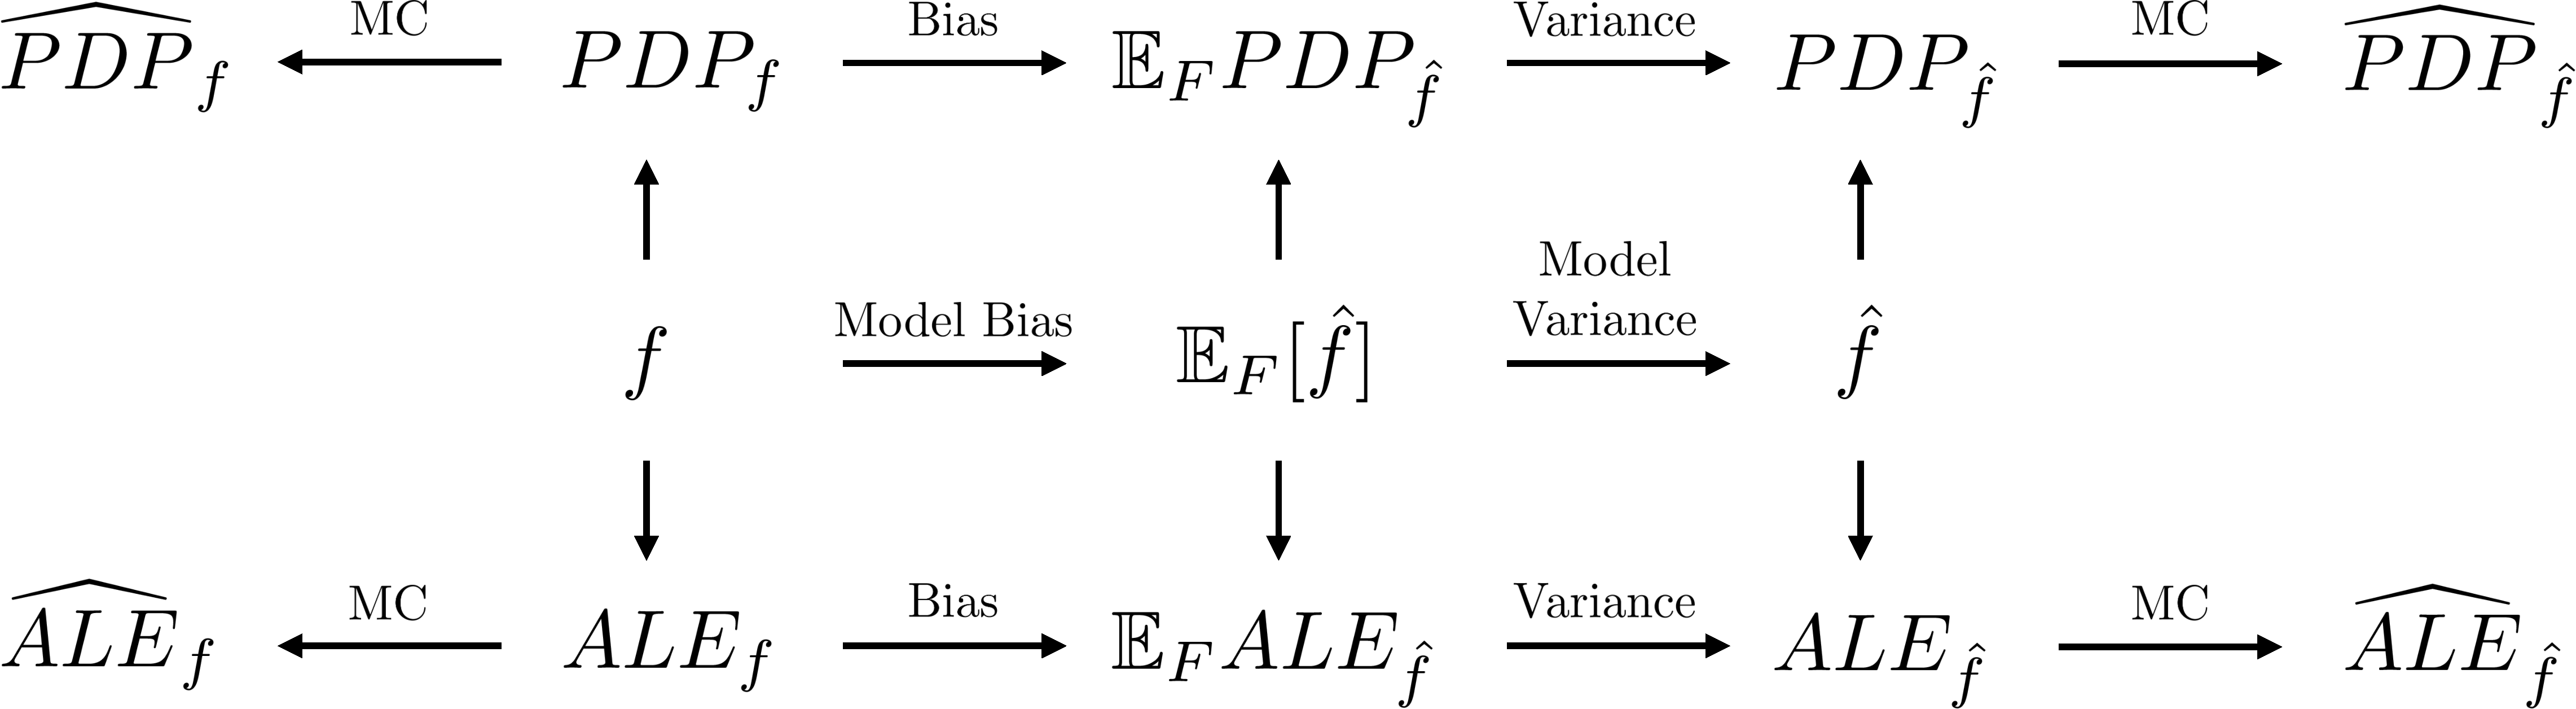
\includegraphics[width=\textwidth]{img/error_graph.pdf}
    \caption{Error chain in feature effect estimation
        (modified, original version can be found in~\cite{molnar_relating_2023})}\label{fig:error-graph}
\end{figure}

\noindent $\mathbb{E}_F$ and $\text{Var}_F$ could be estimated by averaging over
multiple models of the same inducer fitted to $M$ different training data
sets sampled independently from the DGP. We propose the following estimators:
\begin{equation}
    \widehat{\text{MSE}}(x_S; PDP_{f,S}, \widehat{PDP}_{\hat f,S}) = \frac{1}{M} \sum_{m=1}^{M} {(PDP_{f,S}(x_S) - \widehat{PDP}_{\hat f^{(m)},S}(x_S))}^2
    \label{eq:mse-estimator}
\end{equation}
\begin{equation}
    \widehat{\text{Bias}}(x_S; PDP_{f,S}, \widehat{PDP}_{\hat f,S}) = (PDP_{f,S}(x_S) - \frac{1}{M}\sum_{m=1}^M \widehat{PDP}_{\hat{f}^{(m)},S}(x_S))
    \label{eq:bias-estimator}
\end{equation}
\begin{equation}
    \widehat{\text{Variance}}(x_S; \widehat{PDP}_{\hat f,S}) =
    \frac{1}{M-1}\sum_{m=1}^M\left(\widehat{PDP}_{\hat f^{(m)},S}(x_S) - \frac{1}{M}\sum_{m=1}^M \widehat{PDP}_{\hat f^{(m)},S}(x_S)\right)^2
    \label{eq:variance-estimator}
\end{equation}

\noindent Note that these are similar to the approach in~\cite{molnar_relating_2023},
but we do not specify which data points to use for MC integration. The
variance captures both the variance in the model fits and the variance due to
MC integration. To estimate the MC variance, we propose the following estimators:
\begin{equation}
    \widehat{\text{Variance}}_{MC}(x_S; PDP_f, \widehat{PDP}_f) = \frac{1}{K}\sum_{k=1}^K(PDP_f(x_S) - \widehat{PDP}_f^{(k)}(x_S))^2
    \label{eq:mc-variance-estimator-groundtruth}
\end{equation}

\noindent and
\begin{equation}
    \begin{split}
        \widehat{\text{Variance}}_{MC}(x_S; \widehat{PDP}_{\hat{f}}) = \\ \frac{1}{M(K-1)}\sum_{m=1}^M \sum_{k=1}^K
        \left(\widehat{PDP}_{\hat f^{(m)},S}^{(k)}(x_S) - \frac{1}{K}\sum_{k=1}^K \widehat{PDP}_{\hat f^{(m)},S}^{(k)}(x_S)\right)^2
    \end{split}
    \label{eq:mc-variance-estimator-model}
\end{equation}

\noindent For more convenient analysis of the errors, one could also
aggregate them over the marginal distribution of $X_S$ (e.g.,
estimated by averaging over the grid points if chosen appropriately)
to obtain a single error measure per feature effect.

While our definitions are based on the PDP, they can be directly applied to the
ALE as well.

\section{Methodology \& Experimental Set-Up}\label{sec:methodology-set-up}

To address the research question of which data to choose to estimate feature
effects, we conduct a comprehensive simulation study. For different models,
datasets, and dataset sizes, we estimate the feature effects PDP and ALE on
training data, validation data, and in a cross-validated manner. We then
compute the feature effect error as MSE with respect to the ground truth
feature effects and decompose it into bias and variance components. By
comparing these error terms across the different estimation strategies
(training, validation, cross-validation), we aim to provide nuanced empirical
insights into the implications of the data choice on feature effect estimation.
For deeper analysis, we conduct two ablation studies: one decomposing the
feature effect variance into model variance and Monte Carlo variance, and
another examining the impact of the dataset size on the Monte Carlo variance.
In the following, we describe our experimental set-up for the main simulation
study (\textsc{Section~\ref{sec:experiment-main}}) and the ablation studies
(\textsc{Section~\ref{sec:experiment-ablation}}).

\subsection{Main Experiment}\label{sec:experiment-main}

\paragraph{Datasets.}
Building upon \textsc{Section~\ref{sec:test-functions}}, we employ three
distinct datasets of varying complexity for our simulation study:

\begin{itemize}[label=--]
    \item \textbf{SimpleNormalCorrelated} consists of four
          standard-normally distributed features, where the first two
          features exhibit strong correlation ($\rho = 0.9$) while the others are
          independent dummy variables. The target variable is given by this simple
          formula:
          \begin{equation}
              f_1(\boldsymbol{x}) = x_1 + \frac{x_2^2}{2} + x_1 x_2
          \end{equation}
          This test function is inspired by~\cite{liu_model_2018} and aims
          to focus on the impact of correlation and interactions.
    \item \textbf{Friedman1} implements the classical Friedman1 benchmark
          function~\cite{breiman_bagging_1996,friedman_multivariate_1991}
          with seven uniformly distributed features between 0 and 1, all mutually
          independent:
          \begin{equation}
              f_2(\boldsymbol{x}) = 10 \sin(\pi x_1 x_2) + 20(x_3 - \frac{1}{2})^2 + 10 x_4 + 5 x_5
          \end{equation}
          This dataset includes a mix of linear and different non-linear effects with
          interactions.
    \item \textbf{Feynman I.29.16} is based on the Feynman equation I.29.16
          describing wave interference, comprising six independent features. Using
          the refined sampling strategies from Matsubara et al. \cite{matsubara_rethinking_2024},
          two log-uniformly distributed variables on $[0.1, 10]$, two angles uniformly
          distributed over $[0, 2\pi]$, and two uniformly distributed dummy variables on [0,1]:
          \begin{equation}
              f_3(\boldsymbol{x}) = \sqrt{x_1^2 + x_2^2 + 2 x_1 x_2 \cos(\theta_1 - \theta_2)}
          \end{equation}
          This dataset is designed to reflect a physics-based relationship for more real-world relevance.

\end{itemize}

\noindent To generate the datasets, a standard normally distributed noise term $\epsilon$ is added to each function,
scaled by a signal-to-noise ratio of five\footnote{To determine the factor by which the noise is multiplied,
    the standard deviation of the signal is computed over 100'000 randomly drawn samples of $y$ and divided by
    the signal-to-noise ratio of five.}. For each test function, we consider two dataset sizes:
$(n_{train}=1000, n_{val}=250)$ and $(n_{train}=8000, n_{val}=2000)$.

\paragraph{Models.}
We consider a set of seven complementary learners, spanning different modeling
paradigms:

\begin{itemize}[label=--]
    \item \textbf{LinReg}: a simple linear regression model as a baseline.
    \item \textbf{GAM\_OT}: a Generalized Additive Model (GAM) with spline terms
          and tensor splines for first-order interactions, number of splines
          and penalization optimally tuned.
    \item \textbf{GAM\_OF}: as above, but with hyperparameters chosen to overfit.
    \item \textbf{SVM\_OT}: a Support Vector Machine (SVM) with optimally tuned hyperparameters.
    \item \textbf{SVM\_OF}: a Support Vector Machine (SVM) with hyperparameters chosen to overfit.
    \item \textbf{XGBoost\_OT}: an XGBoost model with optimally tuned hyperparameters.
    \item \textbf{XGBoost\_OF}: an XGBoost model with hyperparameters chosen to overfit.
\end{itemize}

\noindent Hyperparameters are pre-selected, i.e.\ carefully hand-picked for overfitting scenarios
and tuned on a different dataset for optimal tuning. Details on the hyperparameters and performances
of the models can be found in \textsc{Appendix~\ref{app:model-hps-perf}}.

\paragraph{Feature effect estimation.}
For the trained models, we estimate the feature effects $\widehat{PDP}_{\hat
        f,S}$ and $\widehat{ALE}_{\hat f,S}$ per feature using
equations~(\ref{eq:pdp-estimate}) and (\ref{eq:ale-estimate-uncentered}). For
Monte Carlo integration, we use for each the full training and validation set
as well as a cross-validation strategy. In the latter case, we use a 5-fold
cross-validation on the combined samples of training and validation set, in
each fold fit the model on four folds, and estimate the feature effects on the
remaining fold. We then average the feature effects over all folds. We also
estimate the ground truth feature effects $\widehat{PDP}_{f,S}$ and
$\widehat{ALE}_{f,S}$ since the complexity of the Feynman equation makes
analytical computation infeasible. For the Monte Carlo integration, we use
10000 samples additionally sampled from the DGP, which introduces only a
negligible additional variance term as we show in (\dots) We use 100 grid
points, defined by the quantiles of the theoretical distribution of $X_S$ to
enable a comparison across feature effects. Additionally, we center the curves
after estimation to have a mean effect of $0$ w.r.t.\ the grid points, and we
omit the first and the last grid point after estimation to avoid boundary
effects especially occuring in ALE plots.

\paragraph{Feature effect errors.} To quantify the error of the estimated feature effects, we compute the MSE of
the estimated model feature effects with respect to the estimated ground truth
features effects, as well as their bias and variance. For that, we use the
estimators defined in equations~(\ref{eq:mse-estimator}) to
(\ref{eq:variance-estimator}), using $\widehat{PDP}_{f,S}$ instead of
$PDP_{f,S}$ as ground truth (analogously for ALE). We repeat each
dataset-size-model combination $M=30$ times to estimate the error terms, where
each repetition involves drawing a new training and validation set from the
DGP, refitting the models, and estimating the feature effects. To aggregate the
errors into a single measure per feature effect, we average the errors over the
marginal distribution of $X_S$ by averaging over the grid points.

\subsection{Ablation Experiments}\label{sec:experiment-ablation}

As described earlier, we conduct two ablation studies for more detailed
insights into the Monte Carlo variance.

\paragraph{Variance decomposition study.} The variance of the feature effects estimated with the procedure described in
the main experiment \textsc{Section~\ref{sec:experiment-main}} consists of two
components: the model variance and the variance due to the Monte Carlo
integration. To disentangle these two sources of variance, we aim to
additionally estimate the Monte Carlo variance using the estimator in
equation~(\ref{eq:mc-variance-estimator-model}). This allows us to substract it
from the total variance estimated in the main experiment and obtain the model
variance, giving more nuanced insights into the implications of the data choice
on feature effect estimation. To obtain this estimate, we maintain the set-up
of the main experiment but for each trained model $\hat f^{(m)}$ (plus five
models from CV $\hat f^{(m,1)} - \hat f^{(m,5)}$), we draw $K=30$ new training
and validation sets from the DGP and estimate the feature effects on these sets
plus in a cross-validated manner with the already fitted models. This allows us
to estimate the Monte Carlo variance as in
equation~(\ref{eq:mc-variance-estimator-model}). Since this study is
computationally more expensive, we do this only for XGBoost (OT and OF) with
the same datasets and sizes as in the main experiment.

\paragraph{Impact of dataset size on Monte Carlo variance.} To investigate the impact of the dataset size on the Monte Carlo variance, we
estimate the Monte Carlo variance between the analytical ground truth feature
effects and the estimated ground truth feature effects on different dataset
sizes. As estimator for the Monte Carlo variance, we use
equation~(\ref{eq:mc-variance-estimator-groundtruth}). With this approach, we
entirely omit the model and thus eliminate other error sources such as model
bias and variance (as with a perfect model fit). To estimate the ground truth
feature effects, we use 50 different dataset sizes ranging from $10^1$ to
$10^6$ on a logarithmic scale. Note that we only consider the
SimpleNormalCorrelated and Friedman1 datasets for this study as an analytical
computation of the FeynmanI.29.16 feature effects is infeasible. For other
details, we maintain the set-up of the main experiment.

\section{Results}\label{sec:results}

\subsection{Main Experiment}

\begin{figure}[htbp]
    \centering
    \begin{subfigure}[b]{0.49\textwidth}
        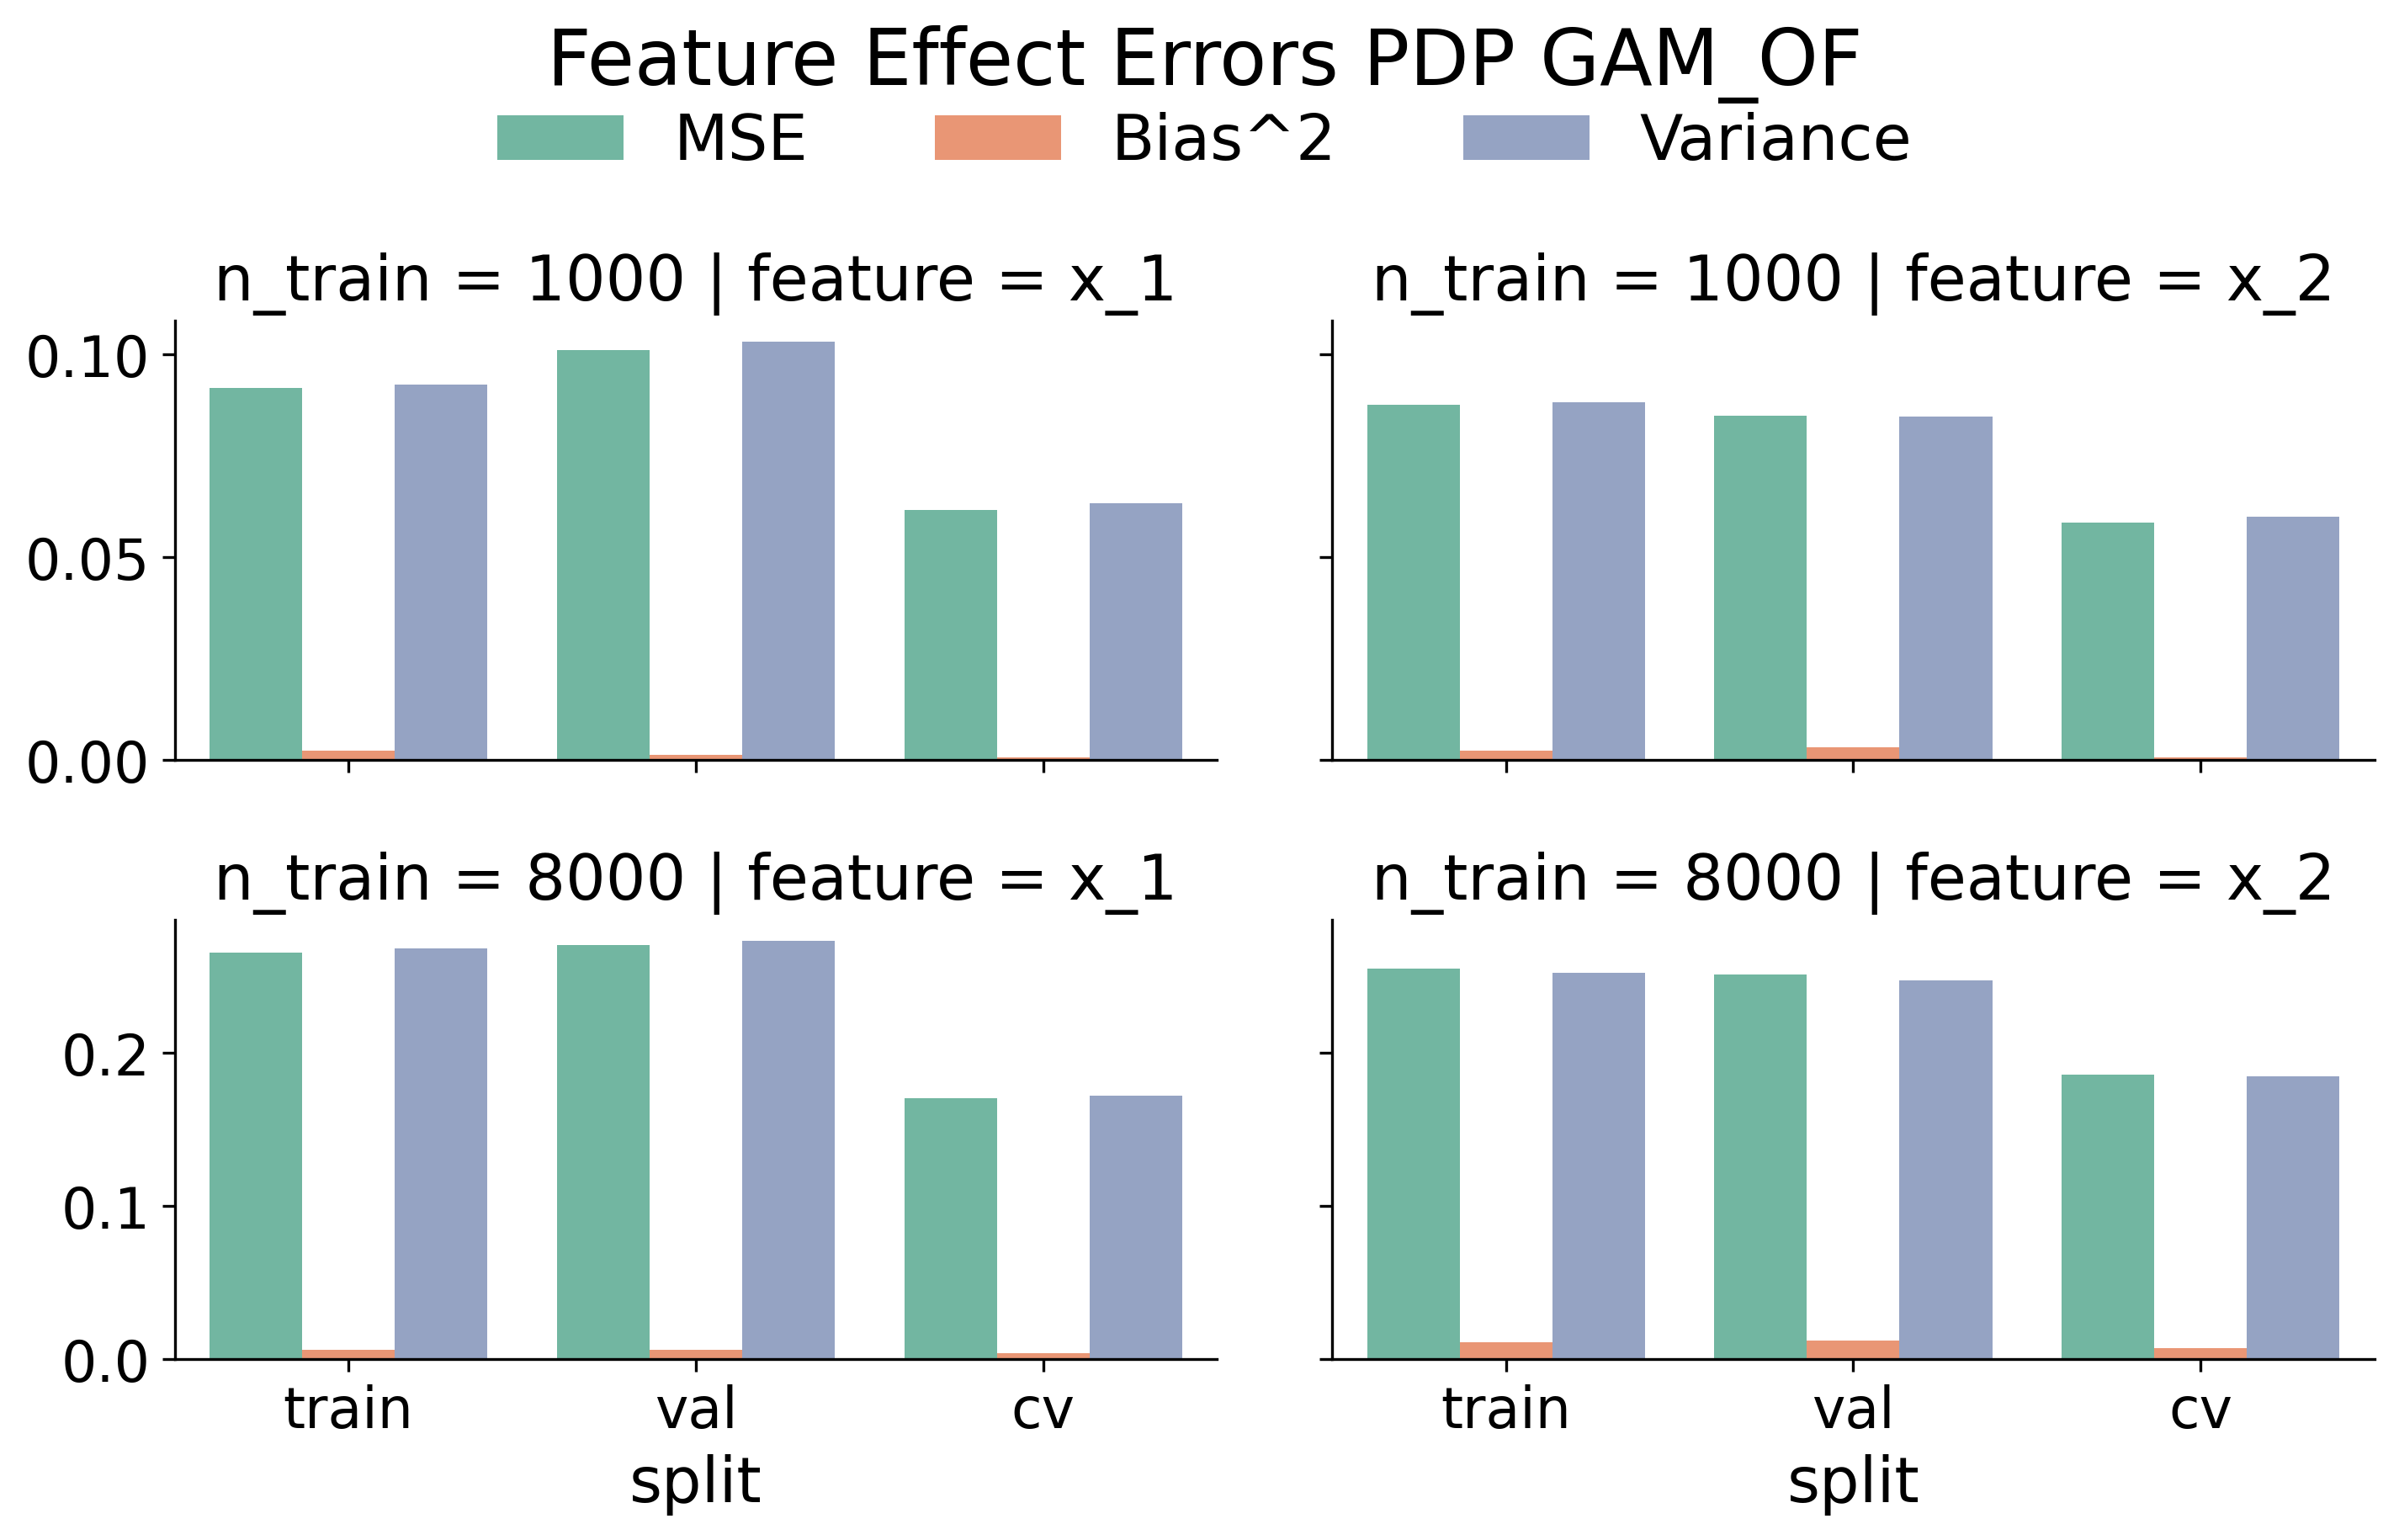
\includegraphics[width=\textwidth]{img/SNC/feature_effect_errors_pdp_GAM_OF.png}
        \caption{GAM\_OF}
    \end{subfigure}
    \hfill
    \begin{subfigure}[b]{0.49\textwidth}
        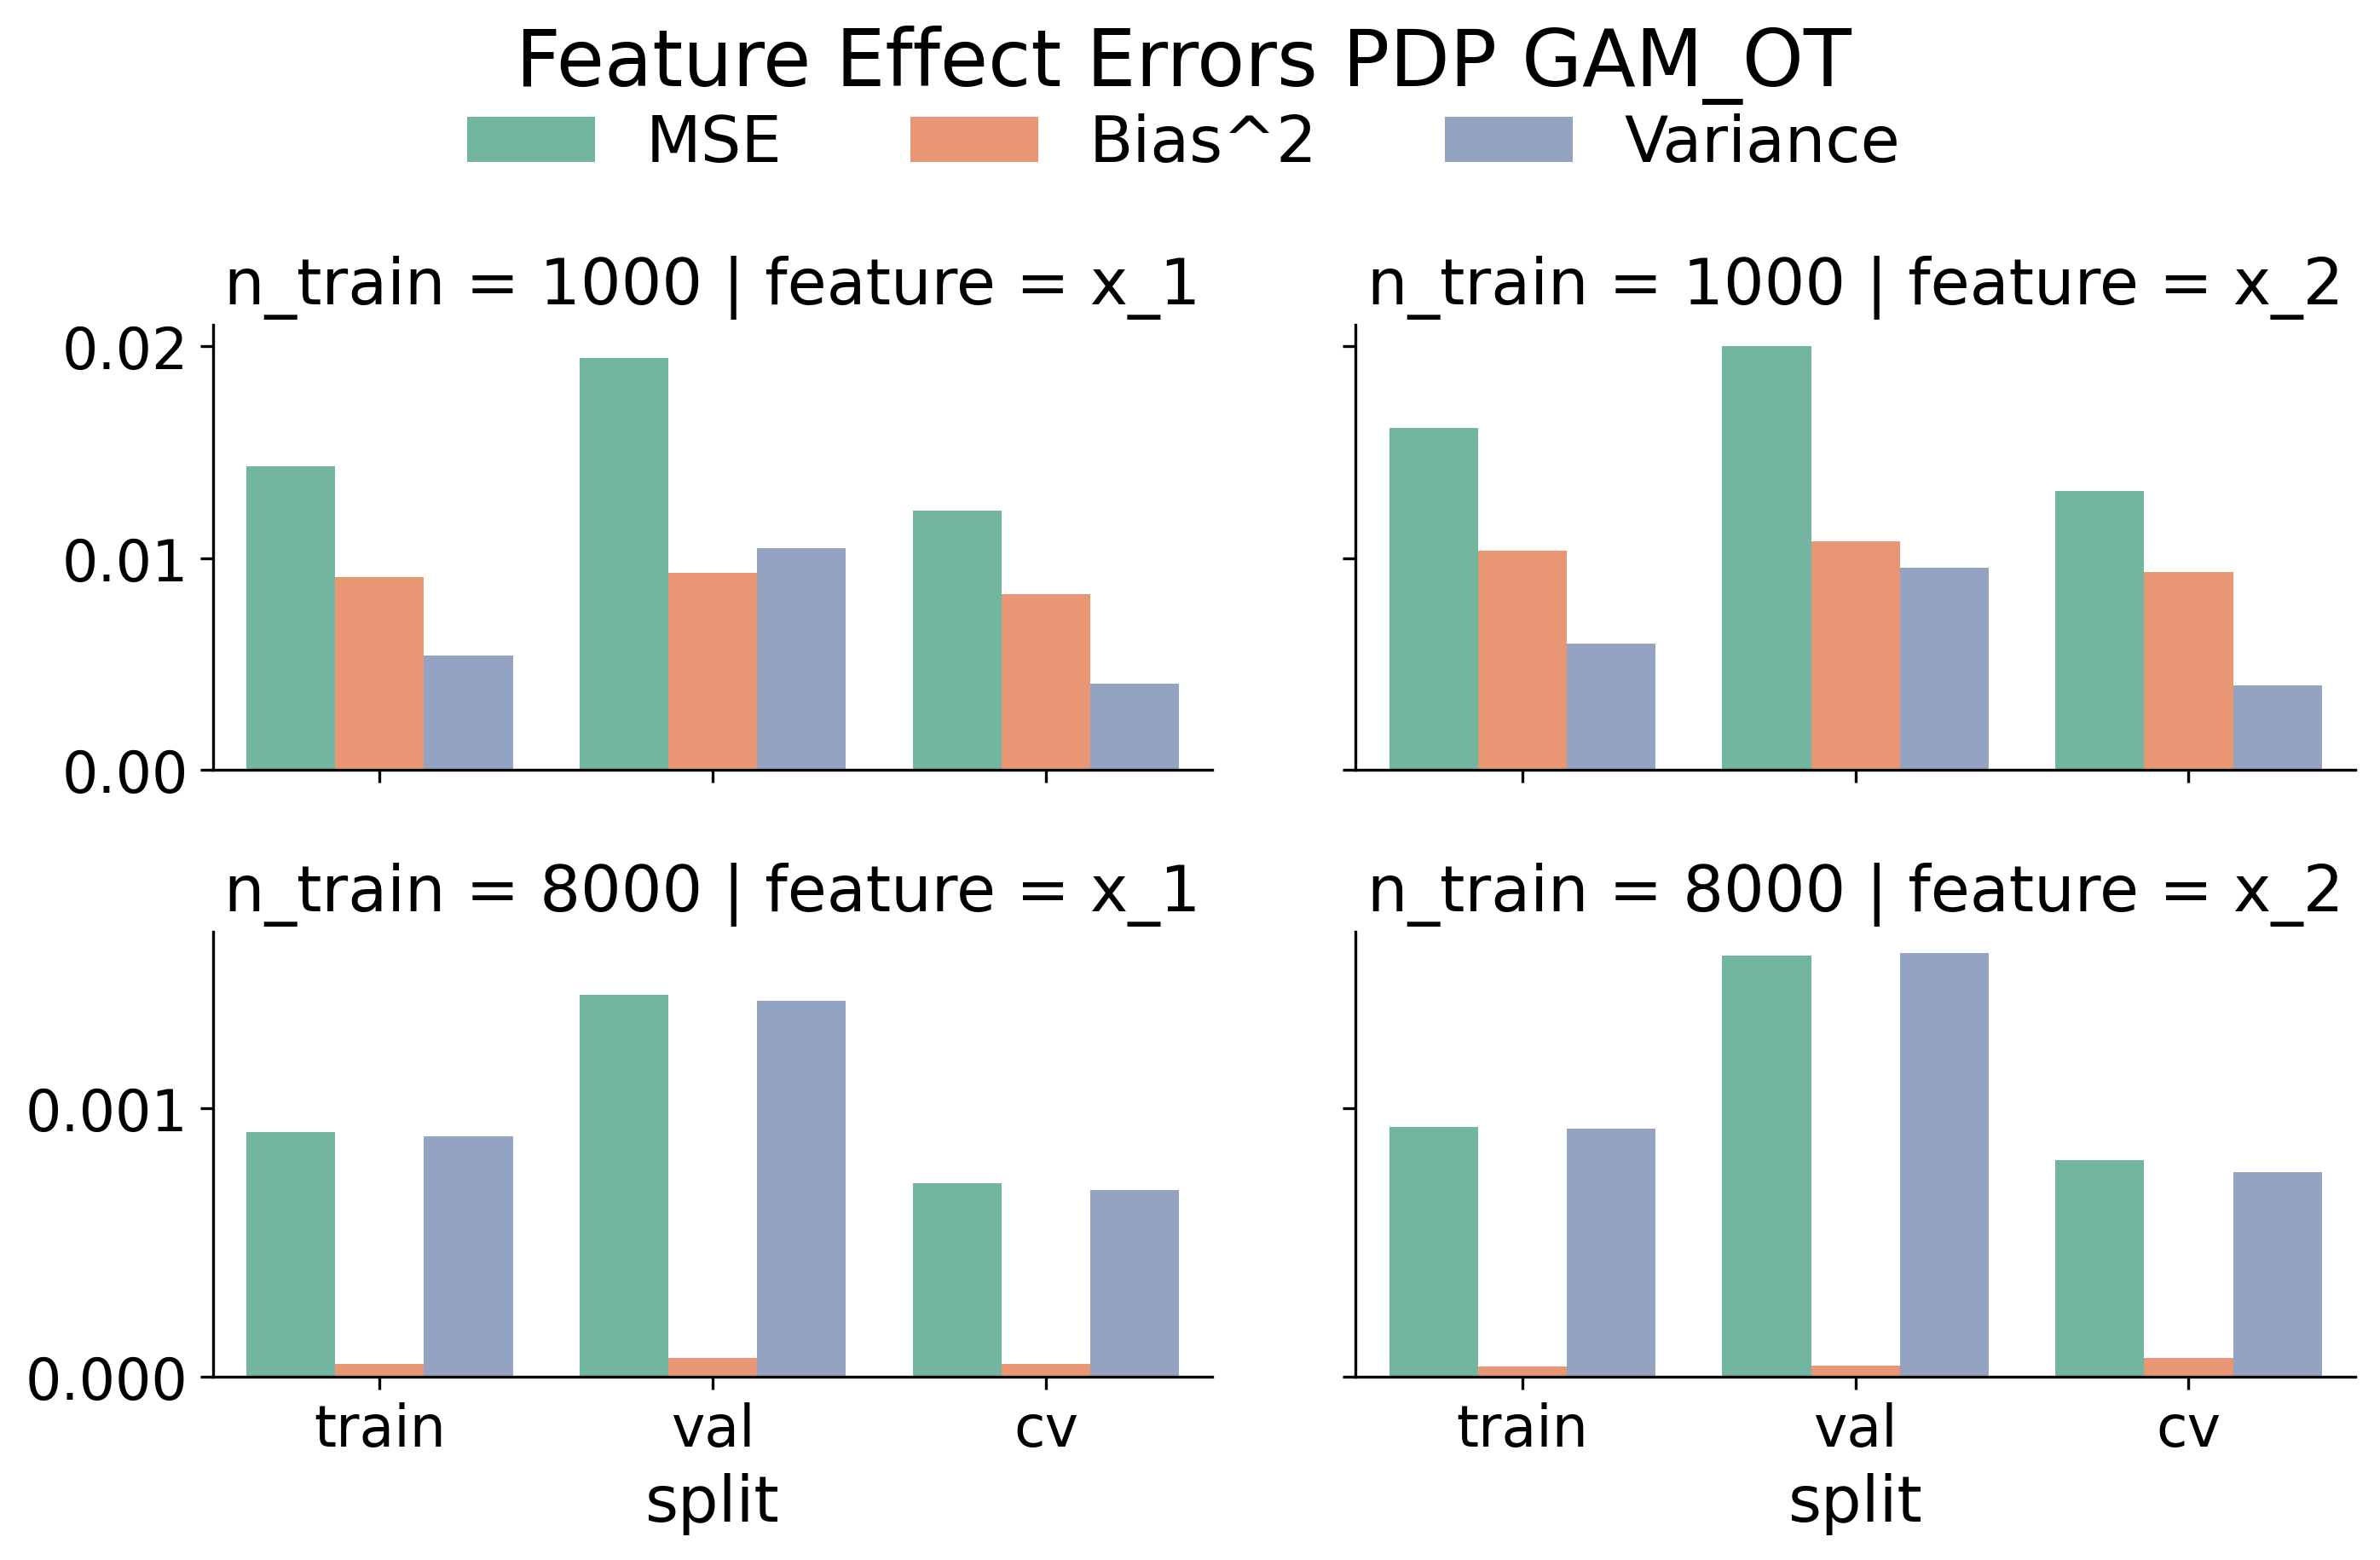
\includegraphics[width=\textwidth]{img/SNC/feature_effect_errors_pdp_GAM_OT.png}
        \caption{GAM\_OT}
    \end{subfigure}
    \\[10pt]
    \hfill
    \begin{subfigure}[b]{0.49\textwidth}
        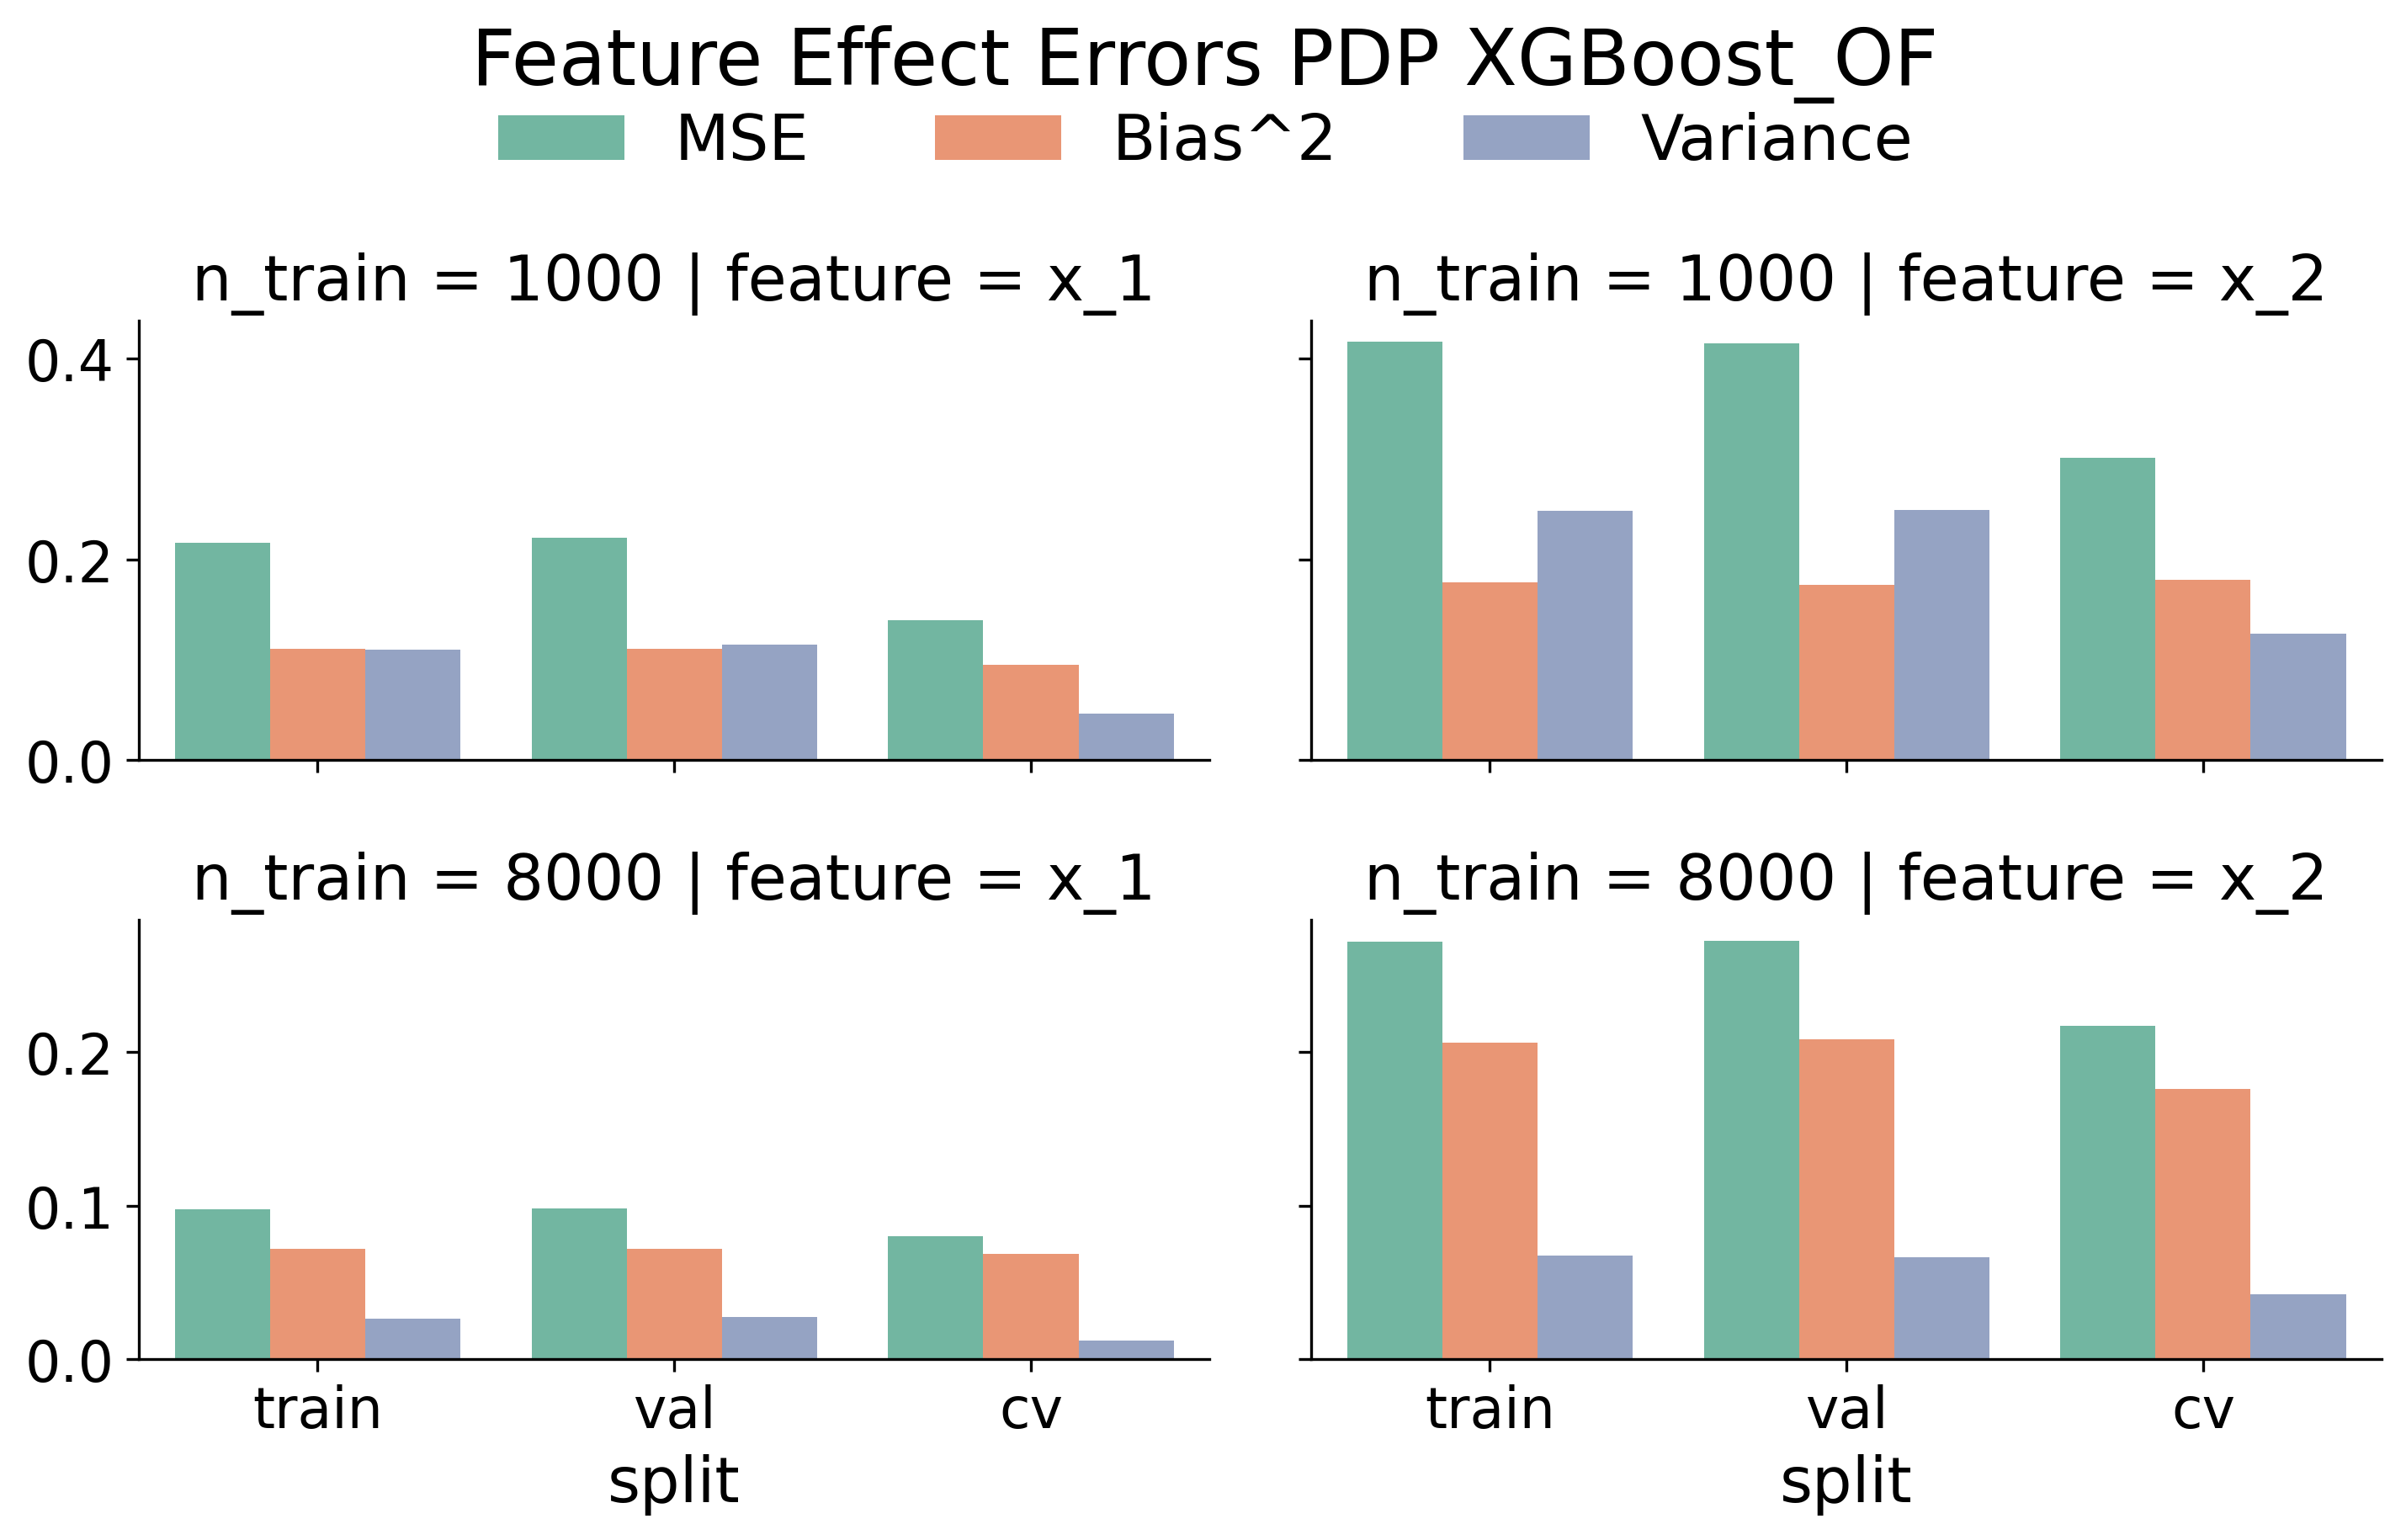
\includegraphics[width=\textwidth]{img/SNC/feature_effect_errors_pdp_XGBoost_OF.png}
        \caption{XGBoost\_OF}
    \end{subfigure}
    \hfill
    \begin{subfigure}[b]{0.49\textwidth}
        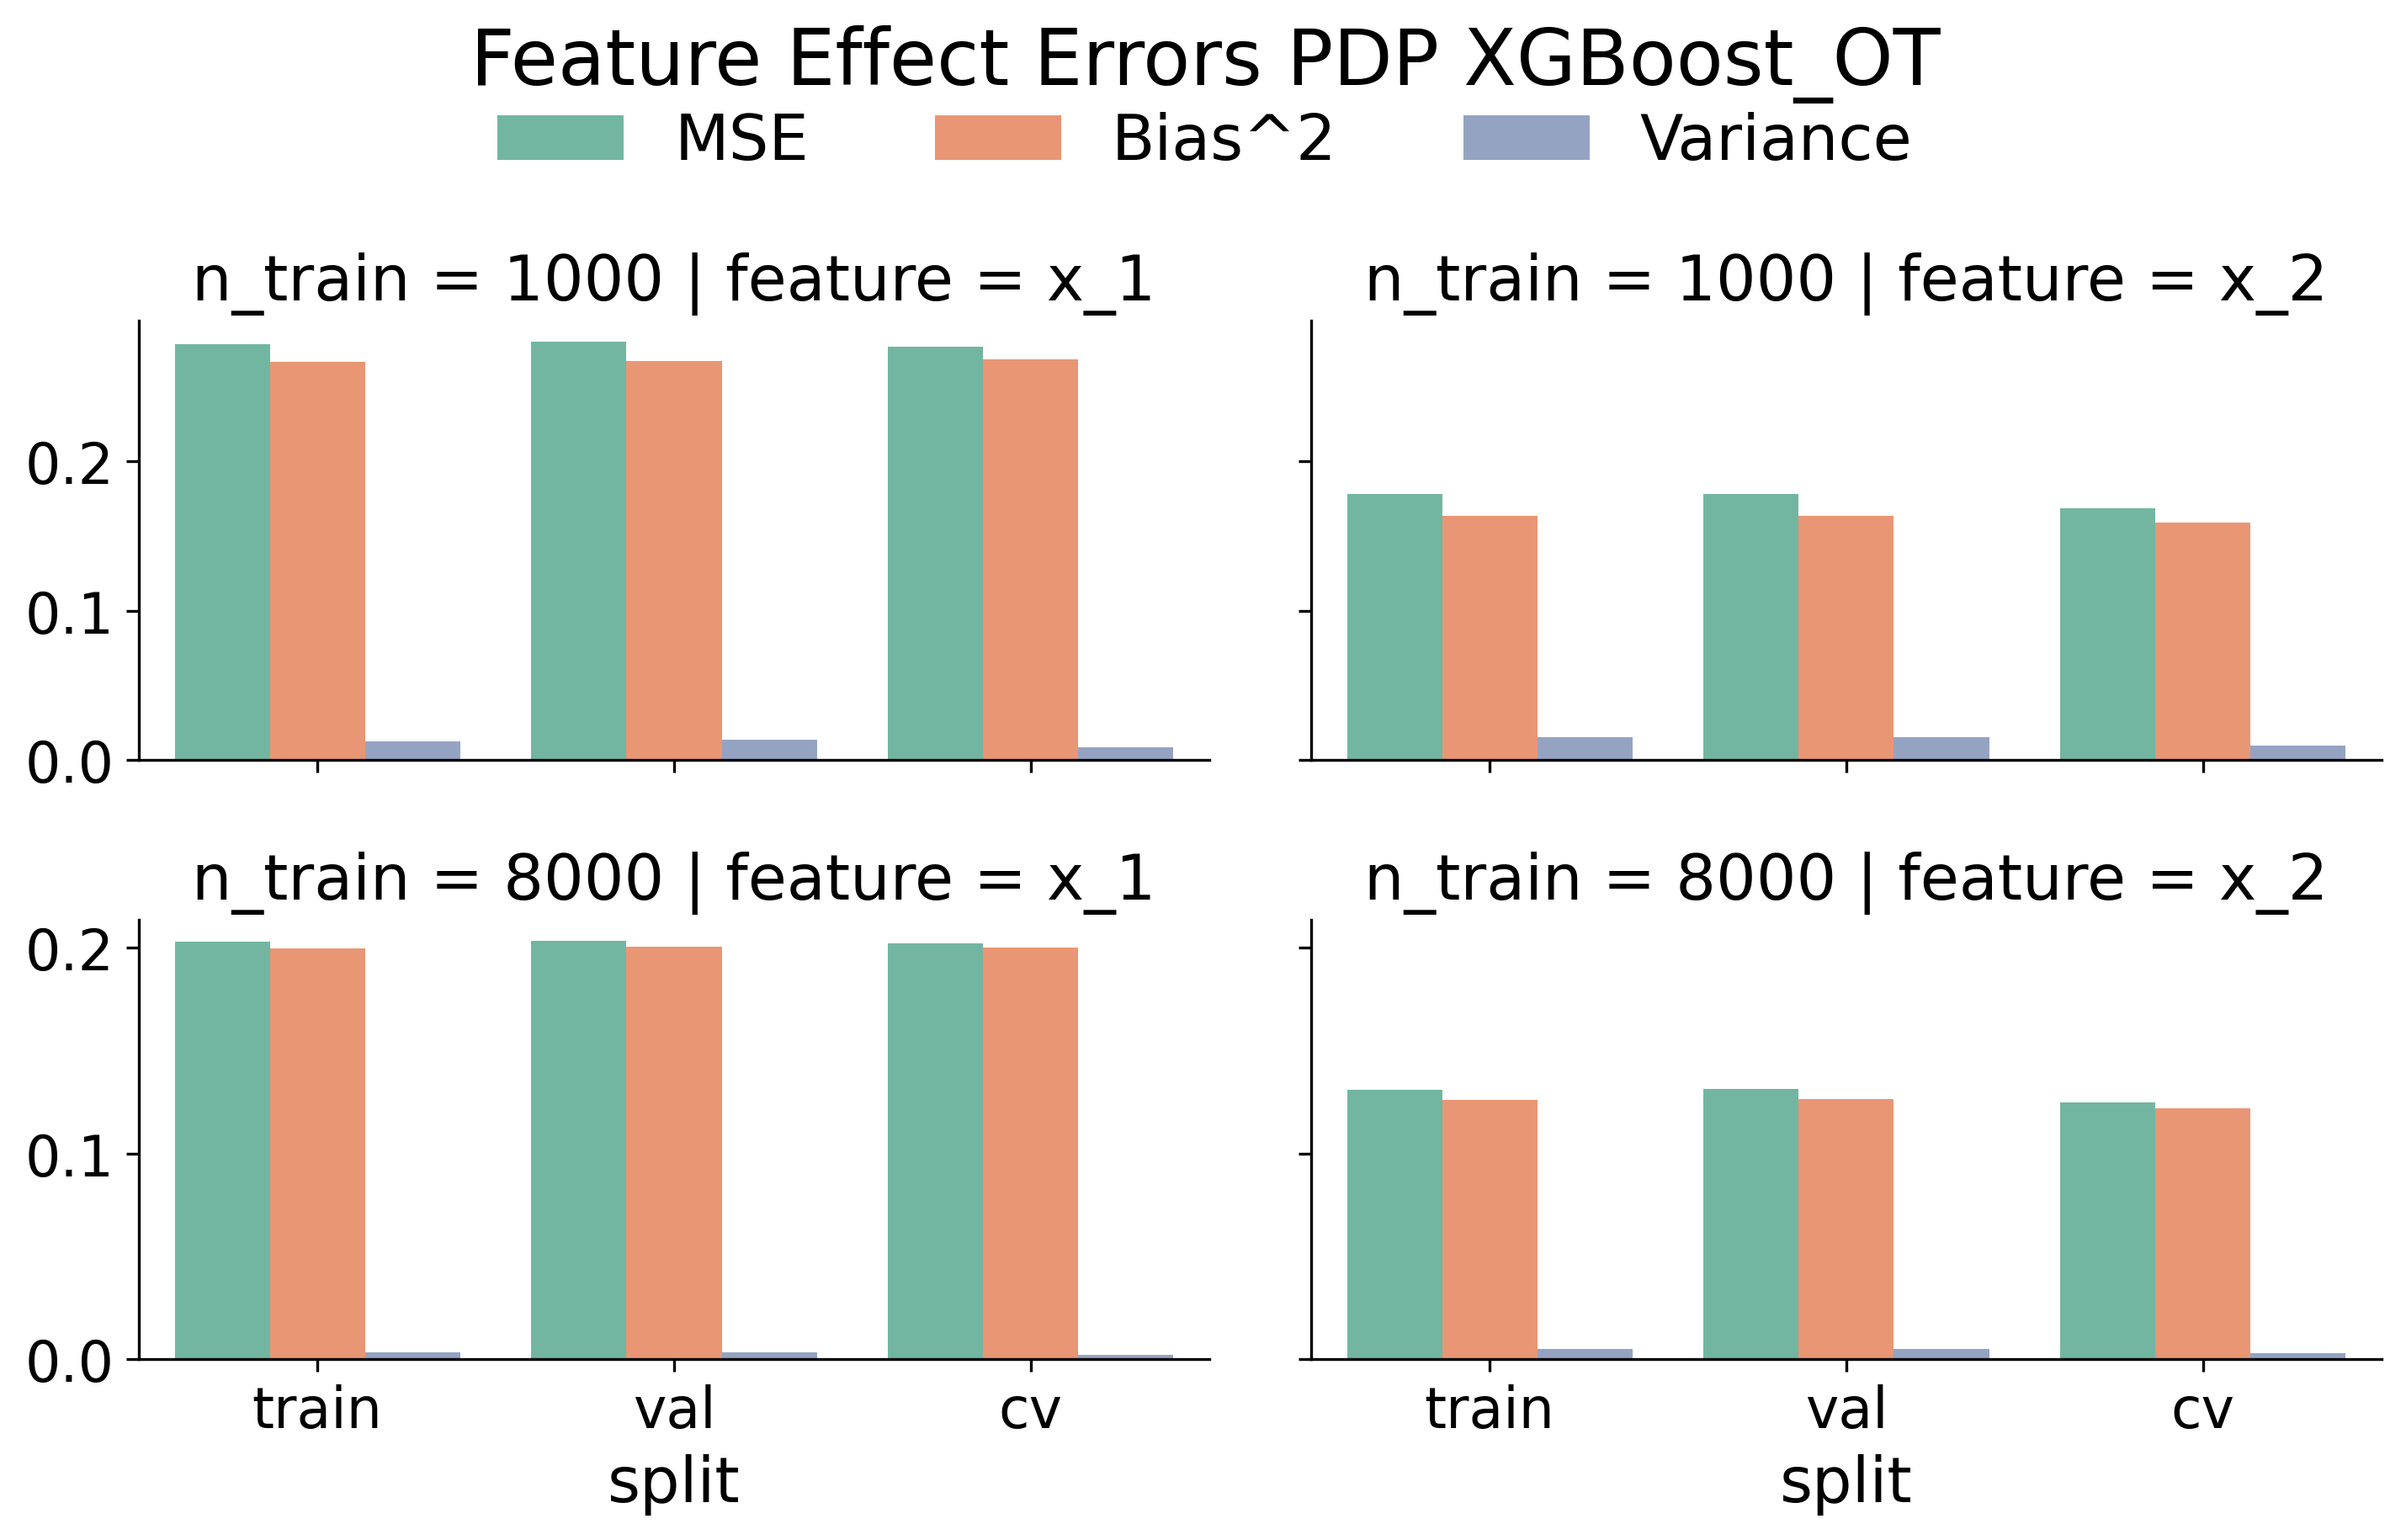
\includegraphics[width=\textwidth]{img/SNC/feature_effect_errors_pdp_XGBoost_OT.png}
        \caption{XGBoost\_OT}
    \end{subfigure}
    \\[10pt]
    \vfill
    \begin{subfigure}[b]{0.49\textwidth}
        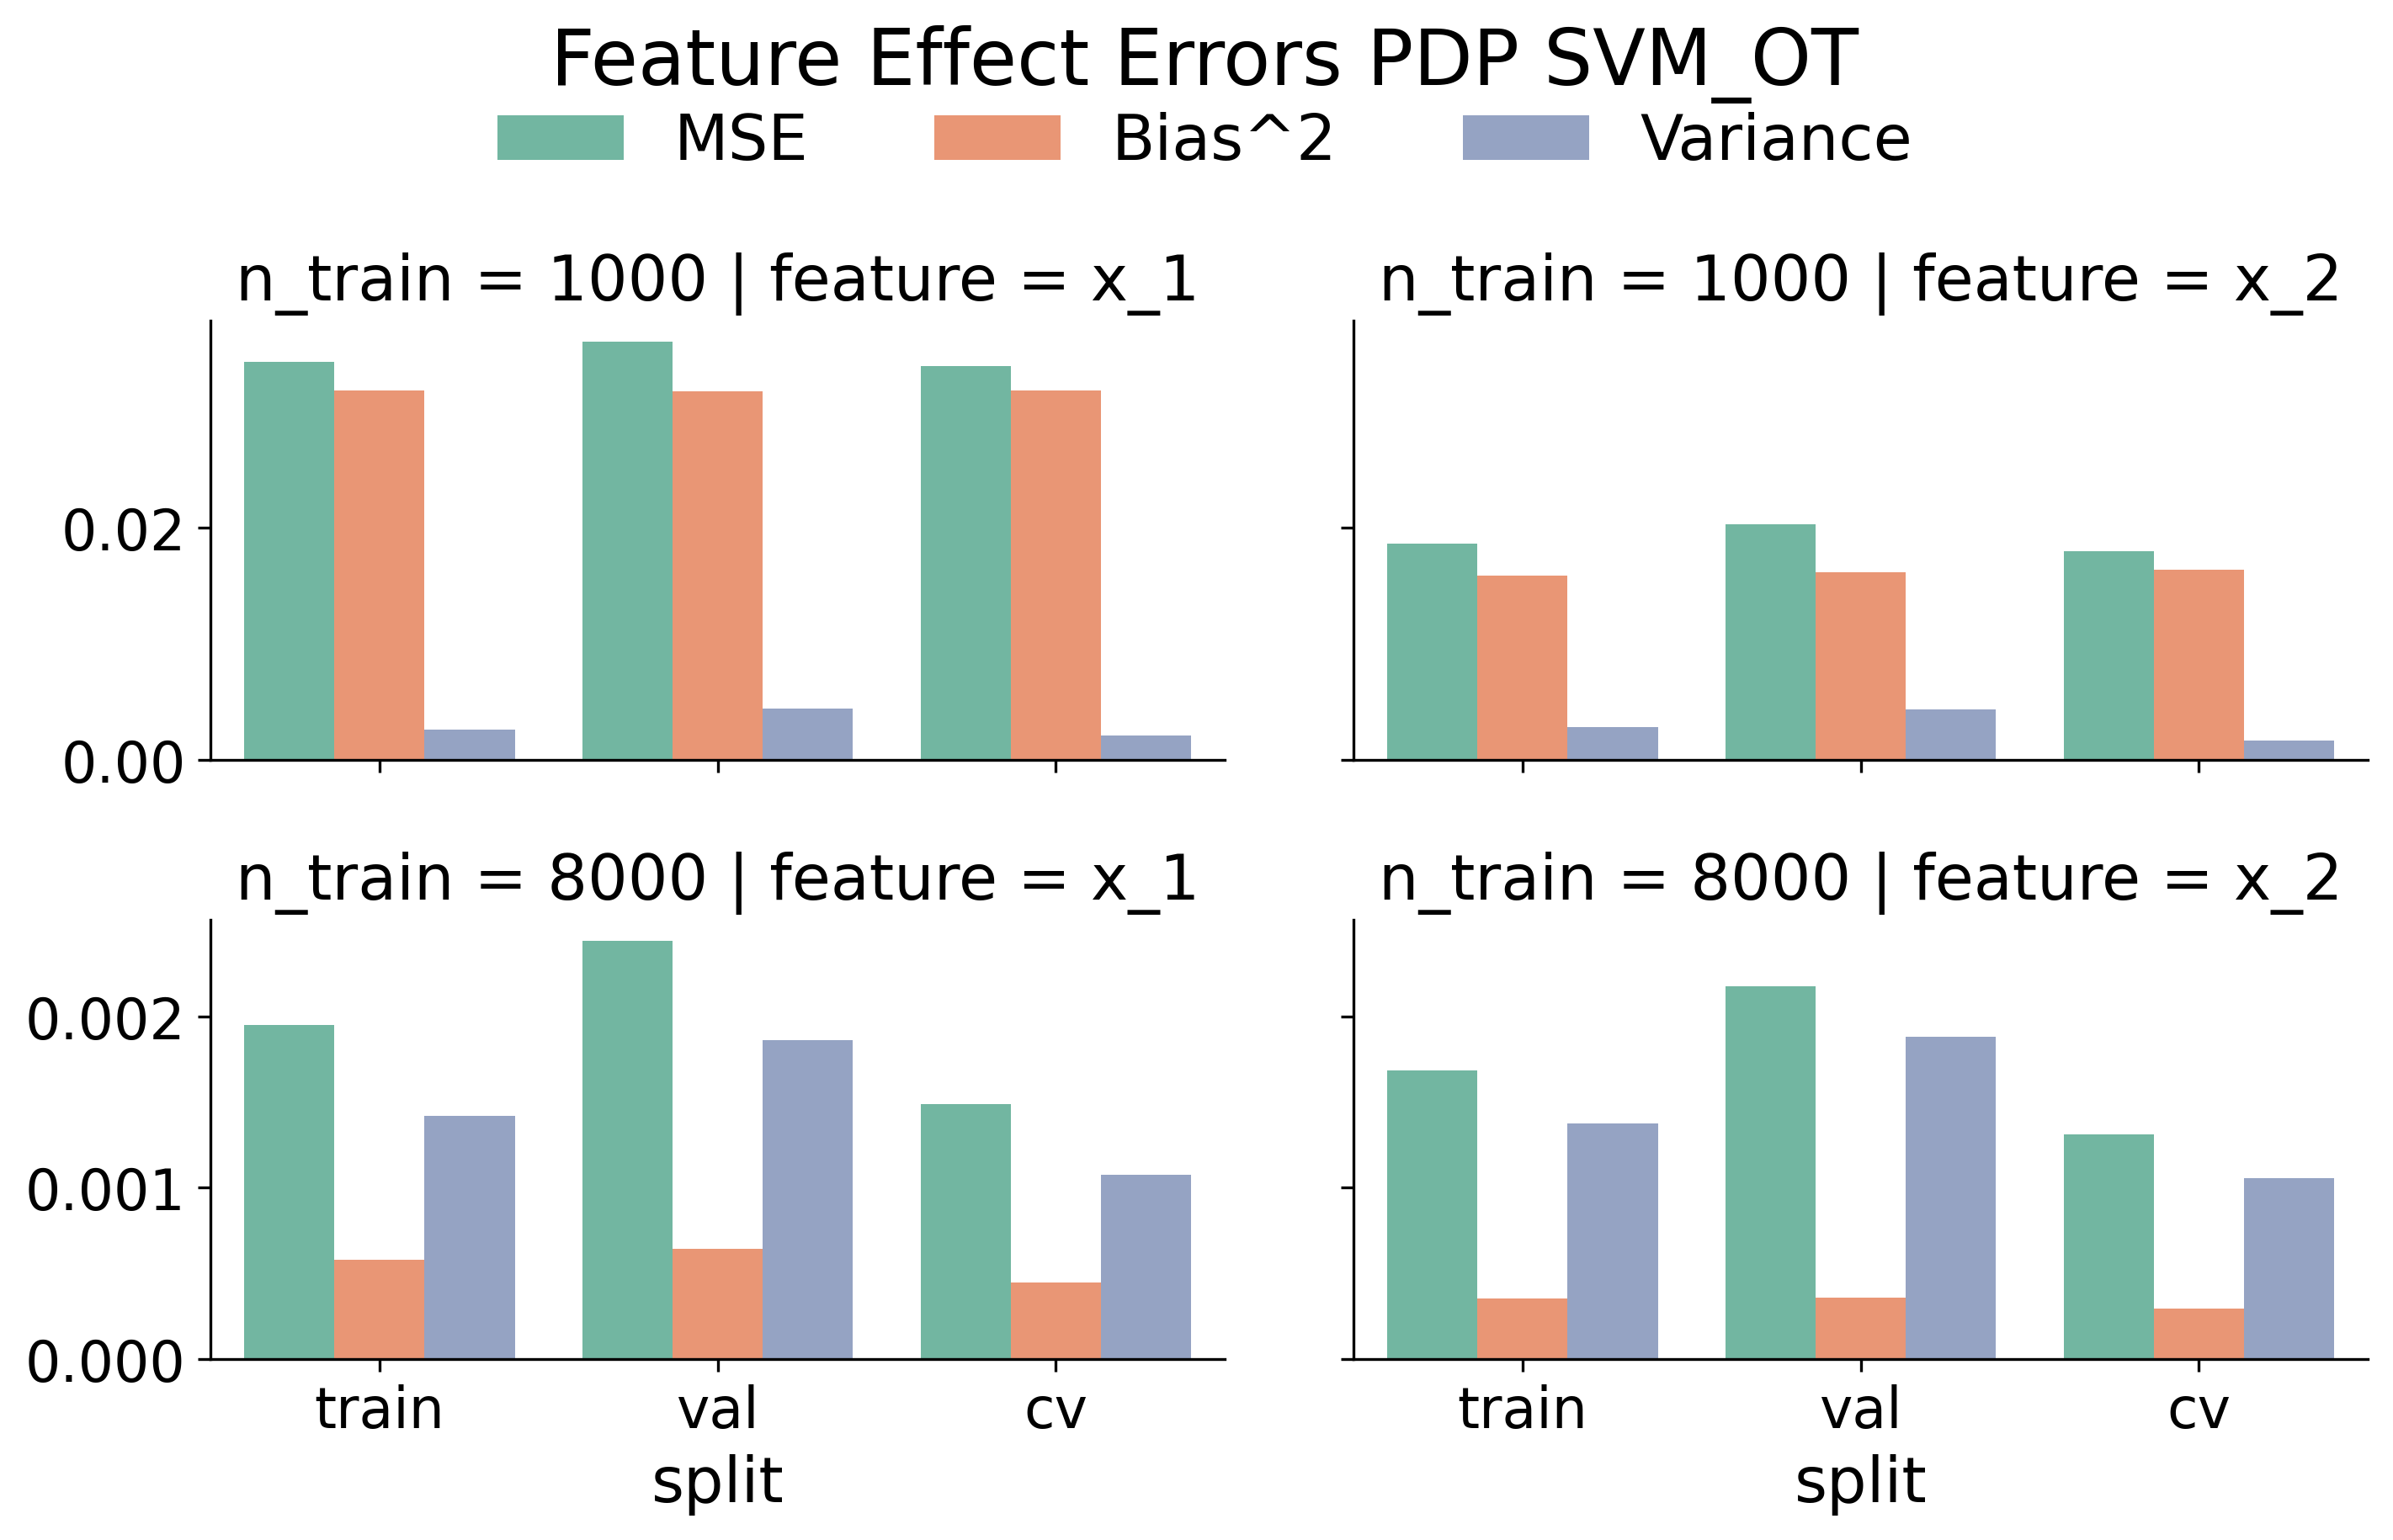
\includegraphics[width=\textwidth]{img/SNC/feature_effect_errors_pdp_SVM_OT.png}
        \caption{SVM\_OT}
    \end{subfigure}
    \caption{Main experiment results for PDP on SimpleNormalCorrelated dataset. \dots}
    \label{fig:pdp-results-snc}
 \end{figure}

 \begin{figure}[htbp]
    \centering
    \begin{subfigure}[b]{0.49\textwidth}
        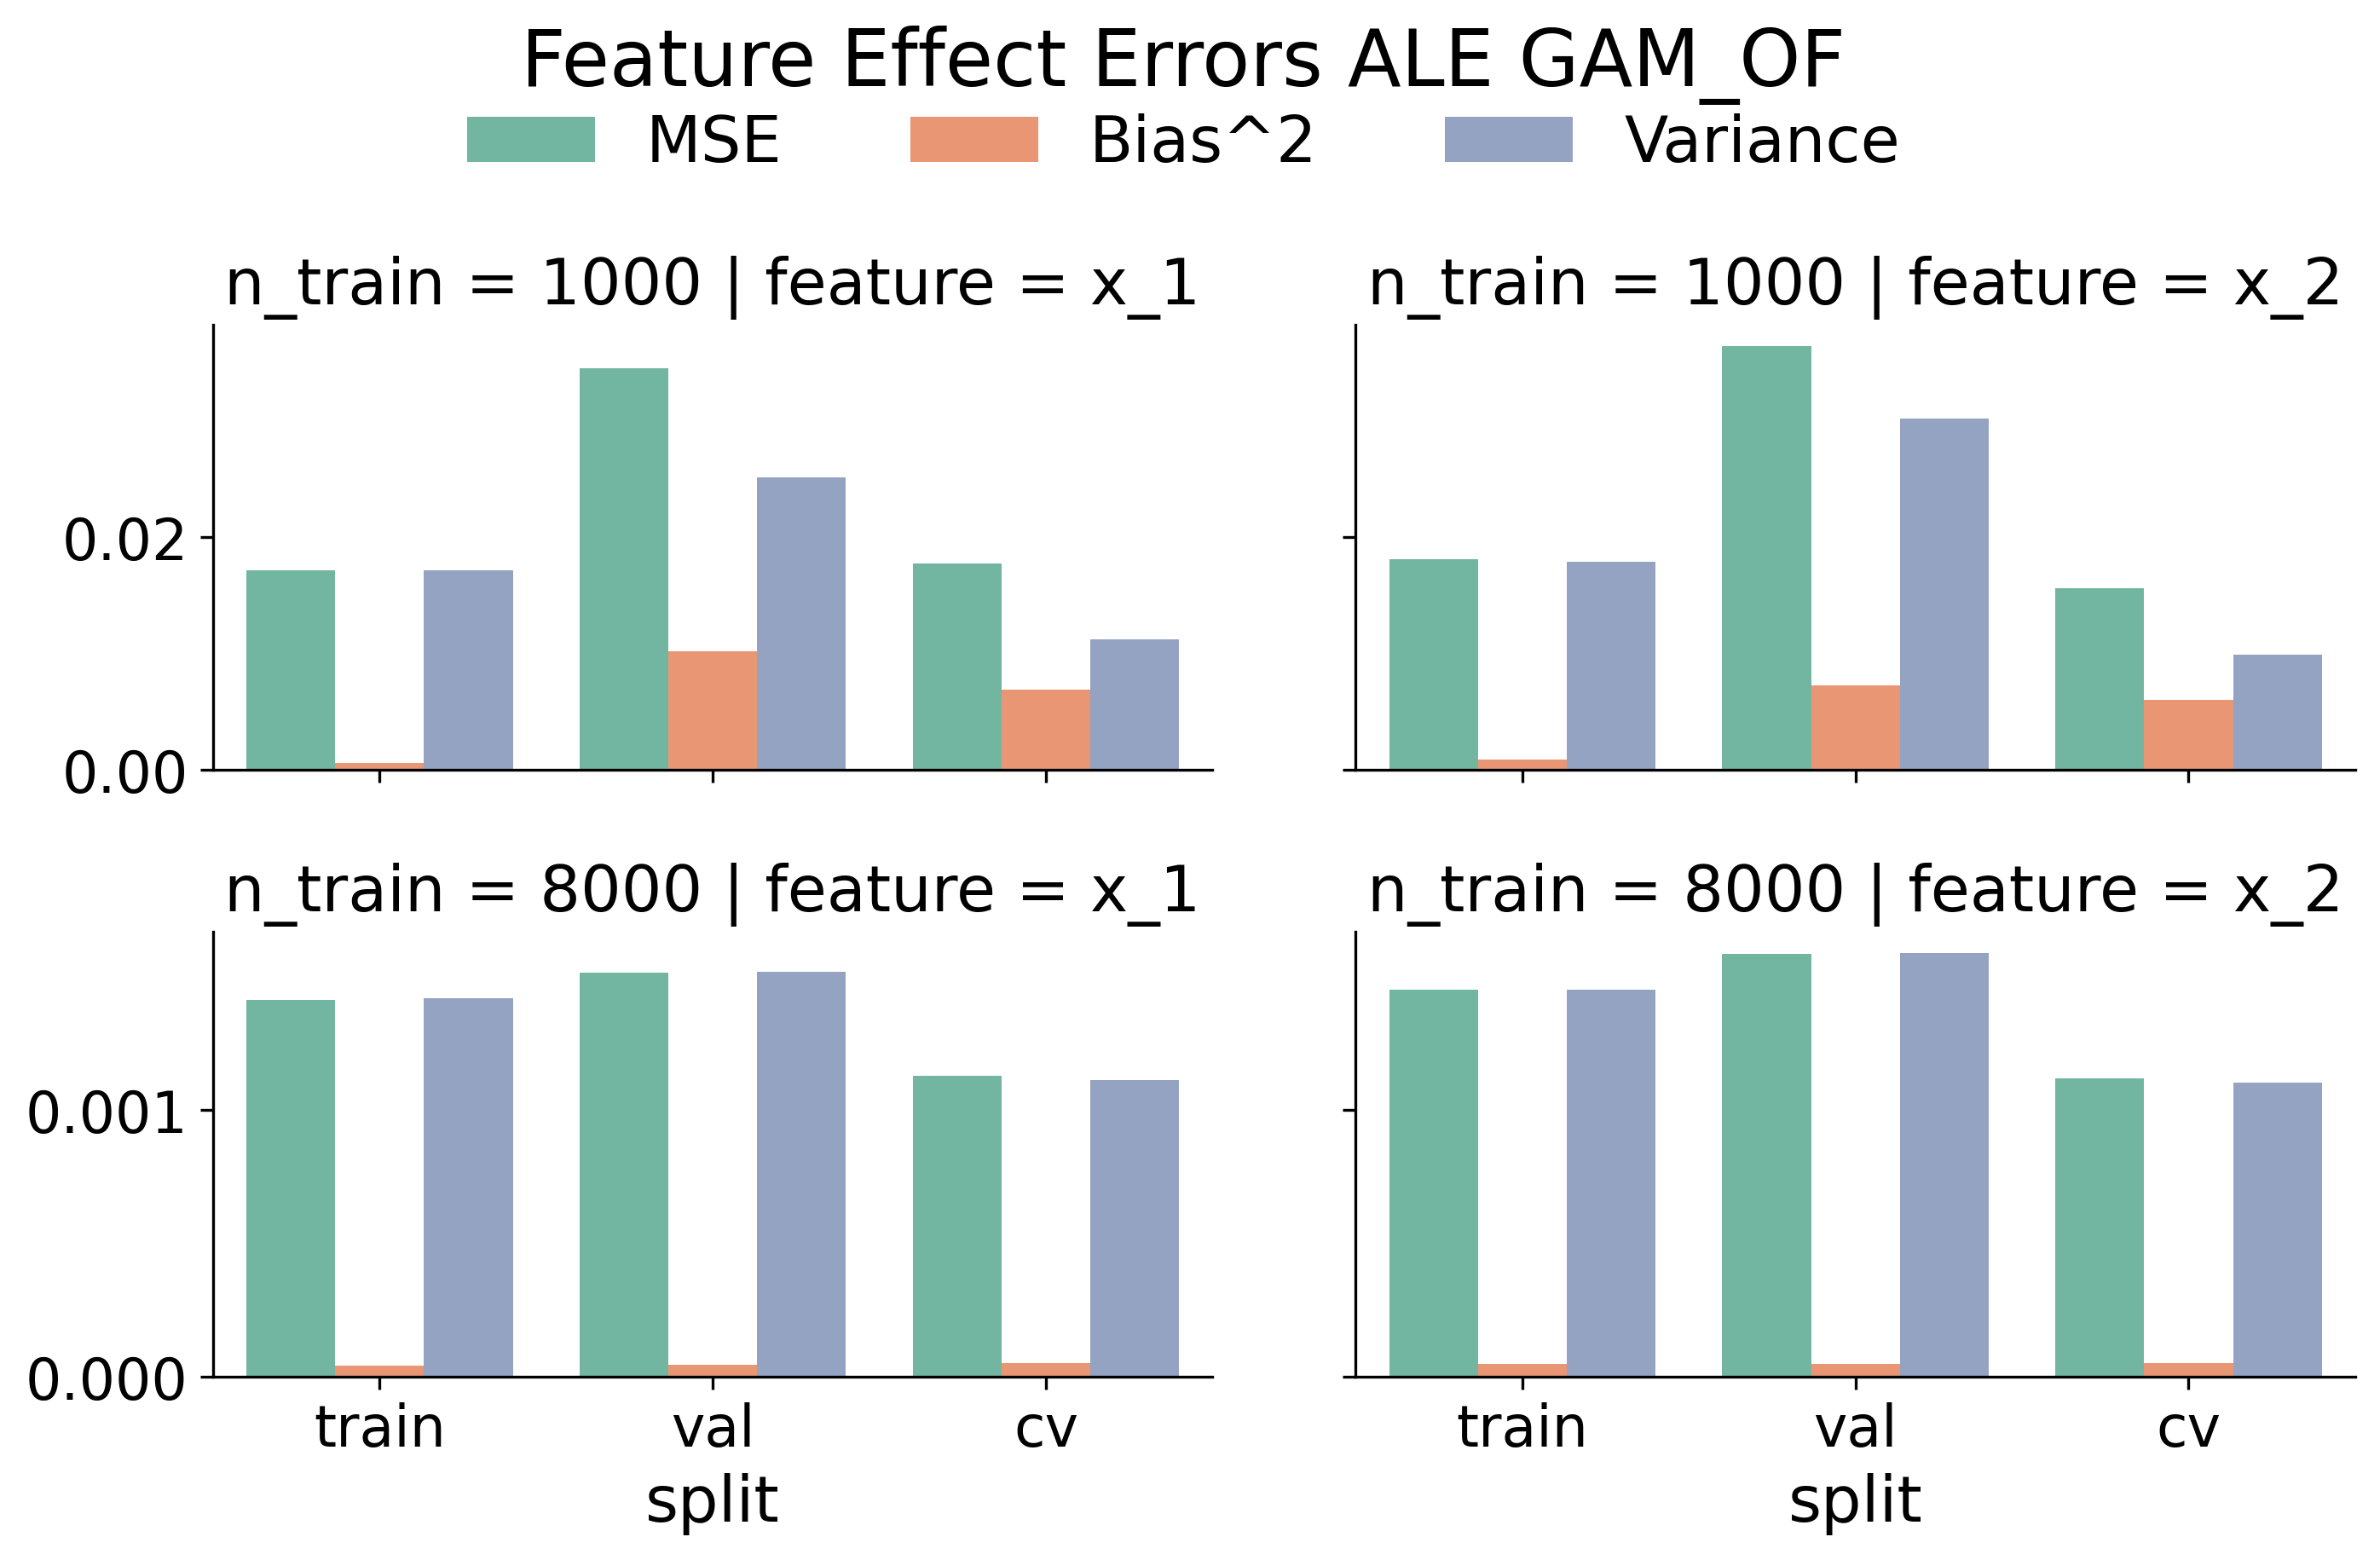
\includegraphics[width=\textwidth]{img/SNC/feature_effect_errors_ale_GAM_OF.png}
        \caption{GAM\_OF}
    \end{subfigure}
    \hfill
    \begin{subfigure}[b]{0.49\textwidth}
        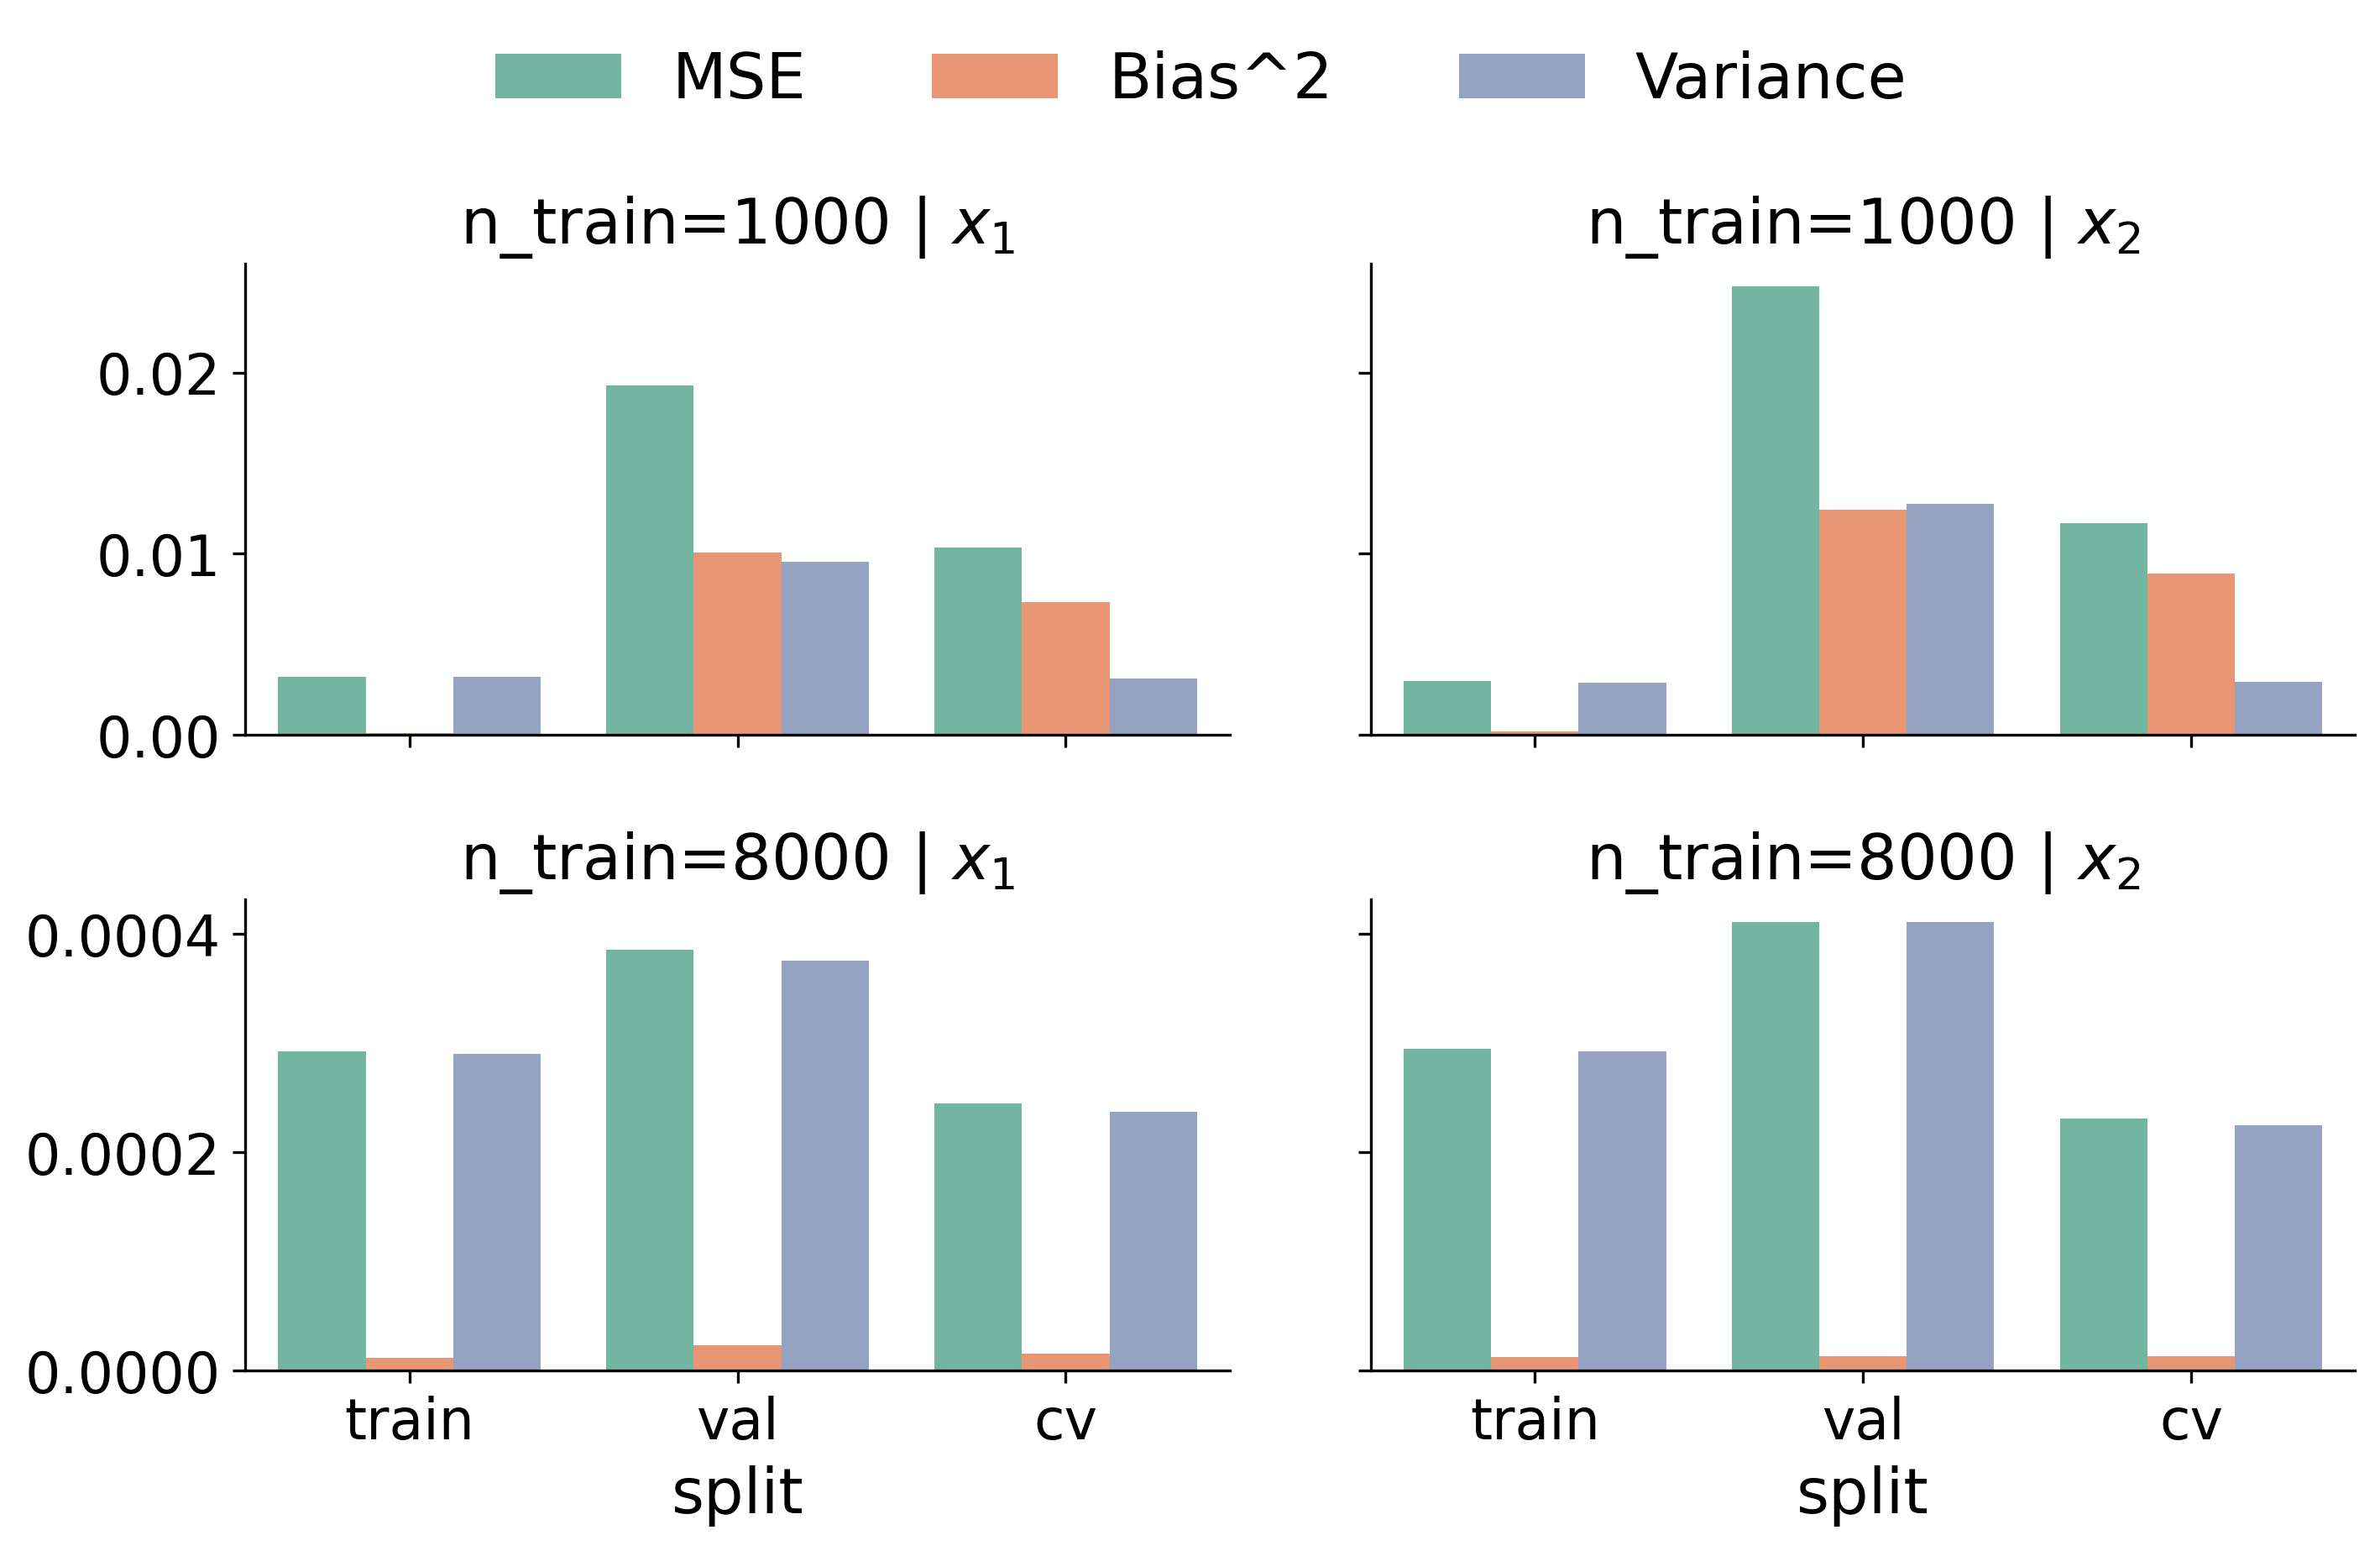
\includegraphics[width=\textwidth]{img/SNC/feature_effect_errors_ale_GAM_OT.png}
        \caption{GAM\_OT}
    \end{subfigure}
    \\[10pt]
    \hfill
    \begin{subfigure}[b]{0.49\textwidth}
        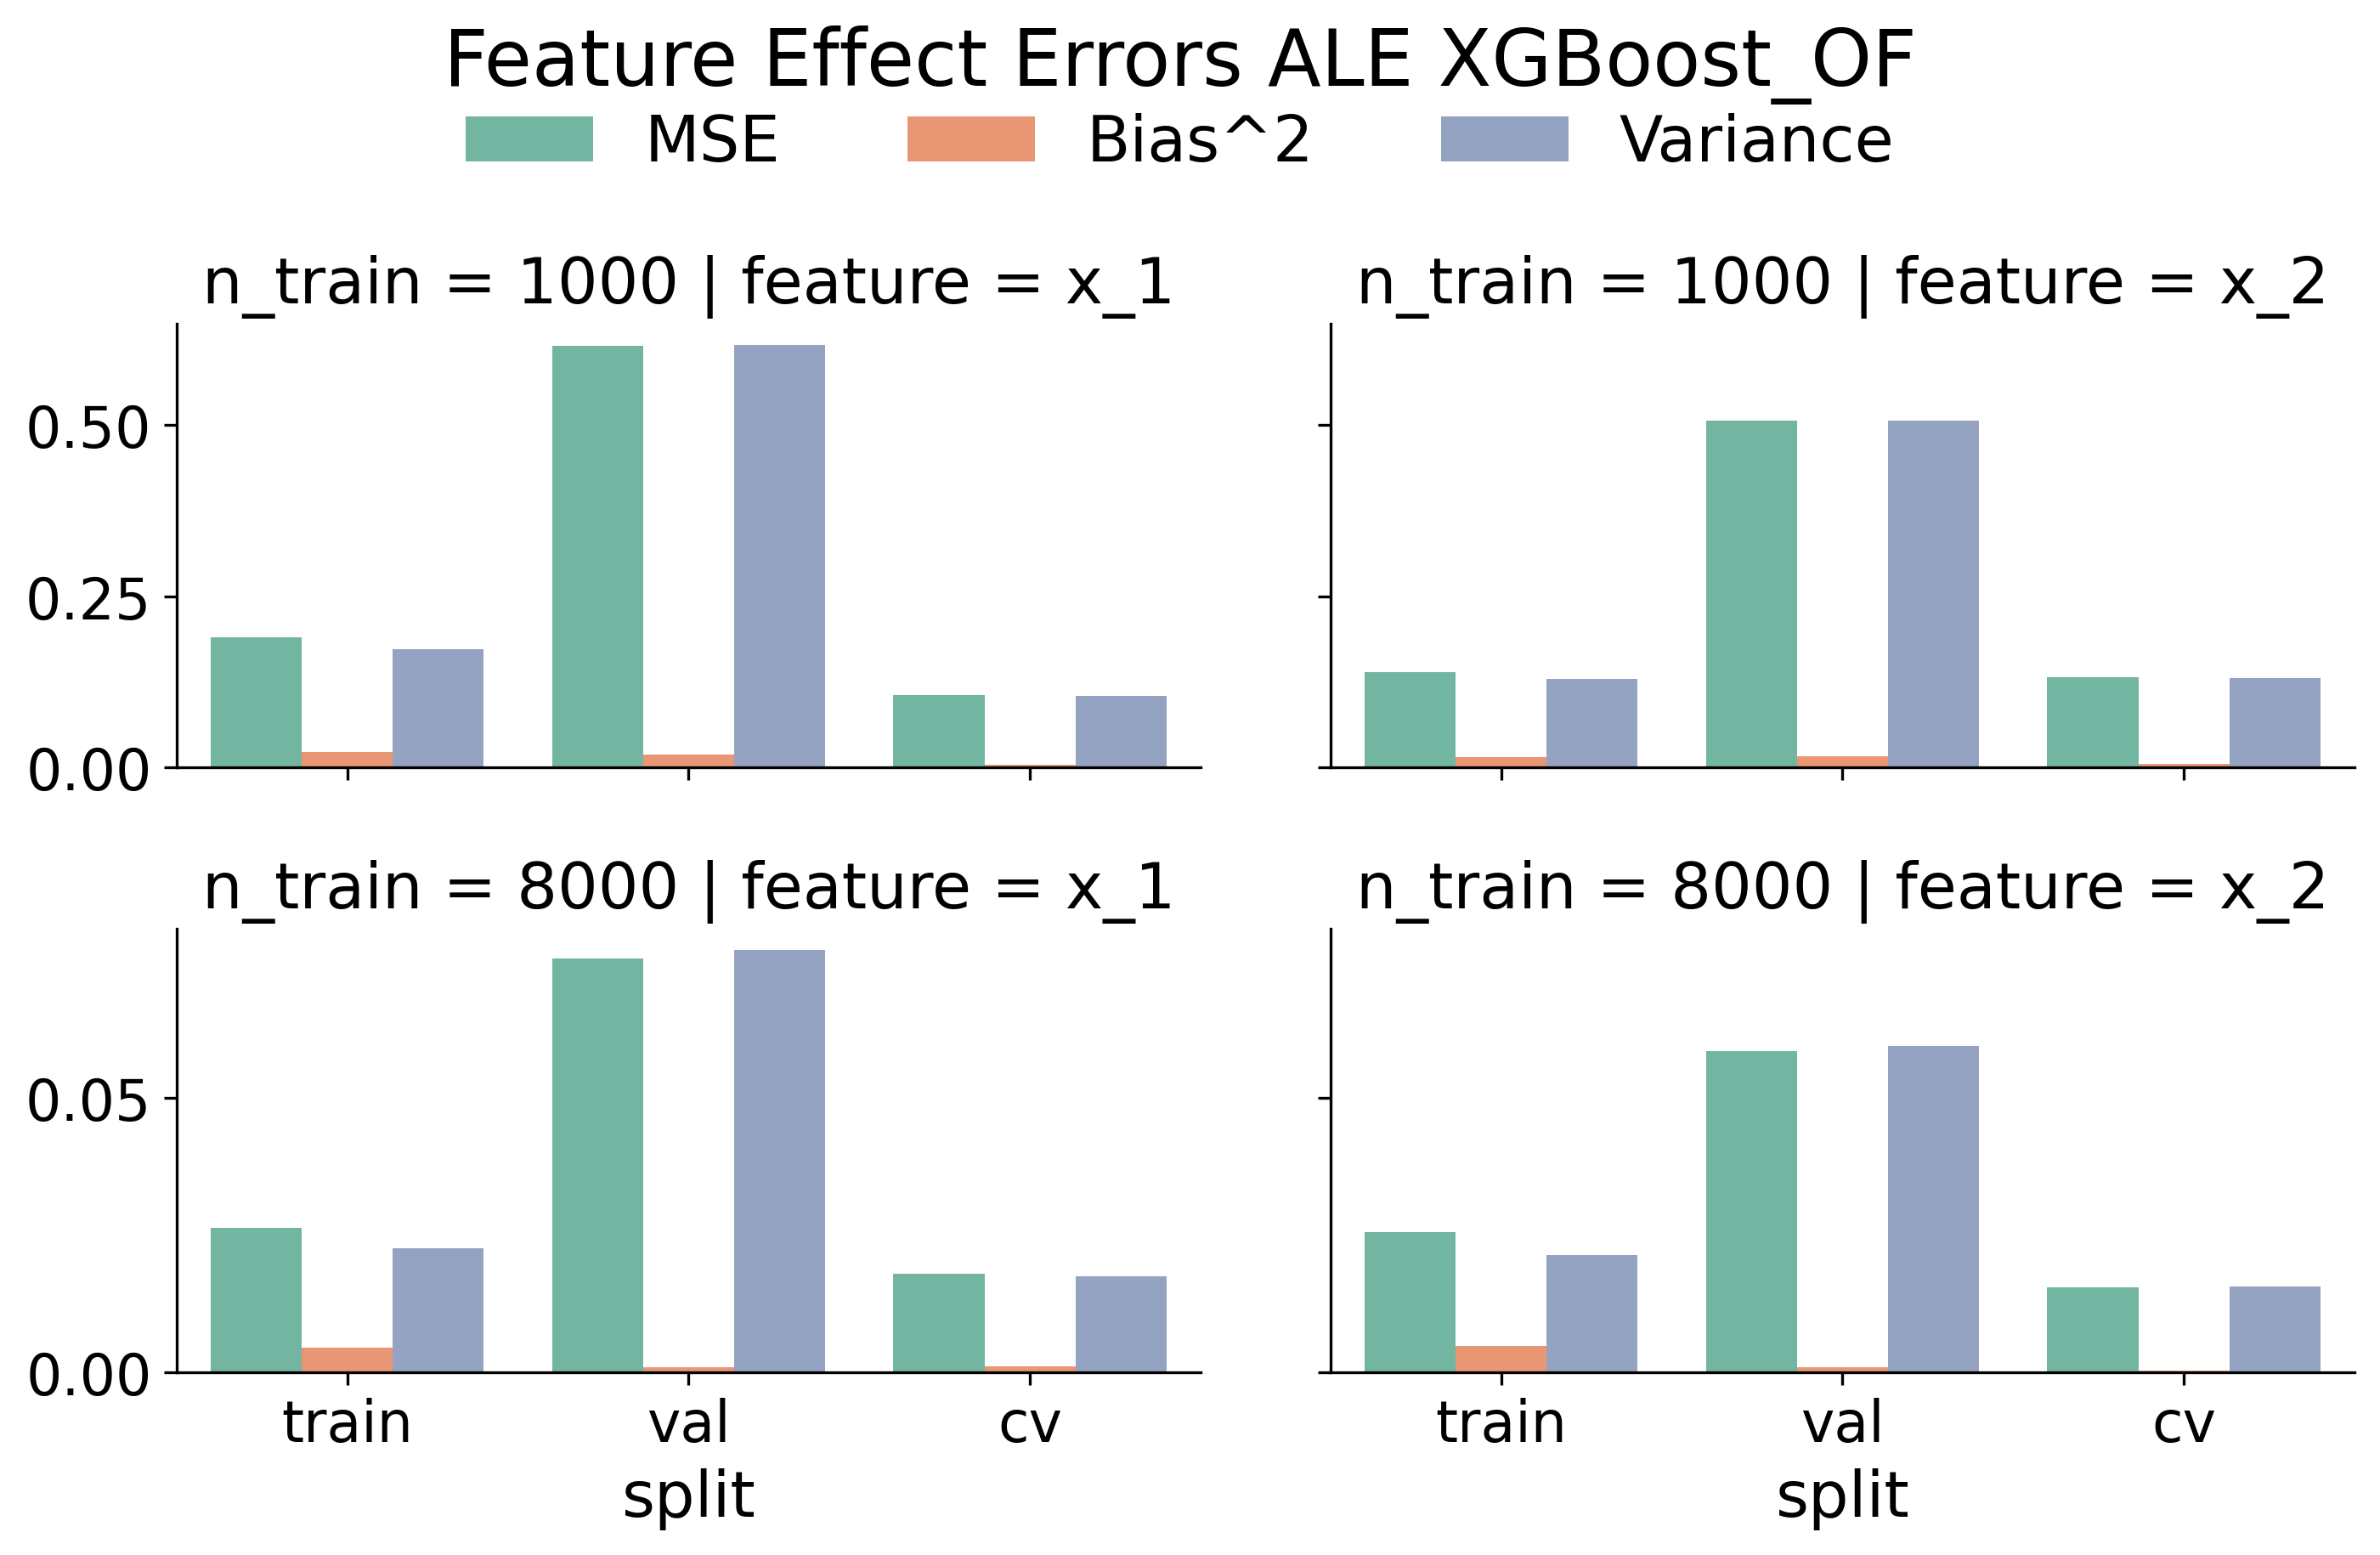
\includegraphics[width=\textwidth]{img/SNC/feature_effect_errors_ale_XGBoost_OF.png}
        \caption{XGBoost\_OF}
    \end{subfigure}
    \hfill
    \begin{subfigure}[b]{0.49\textwidth}
        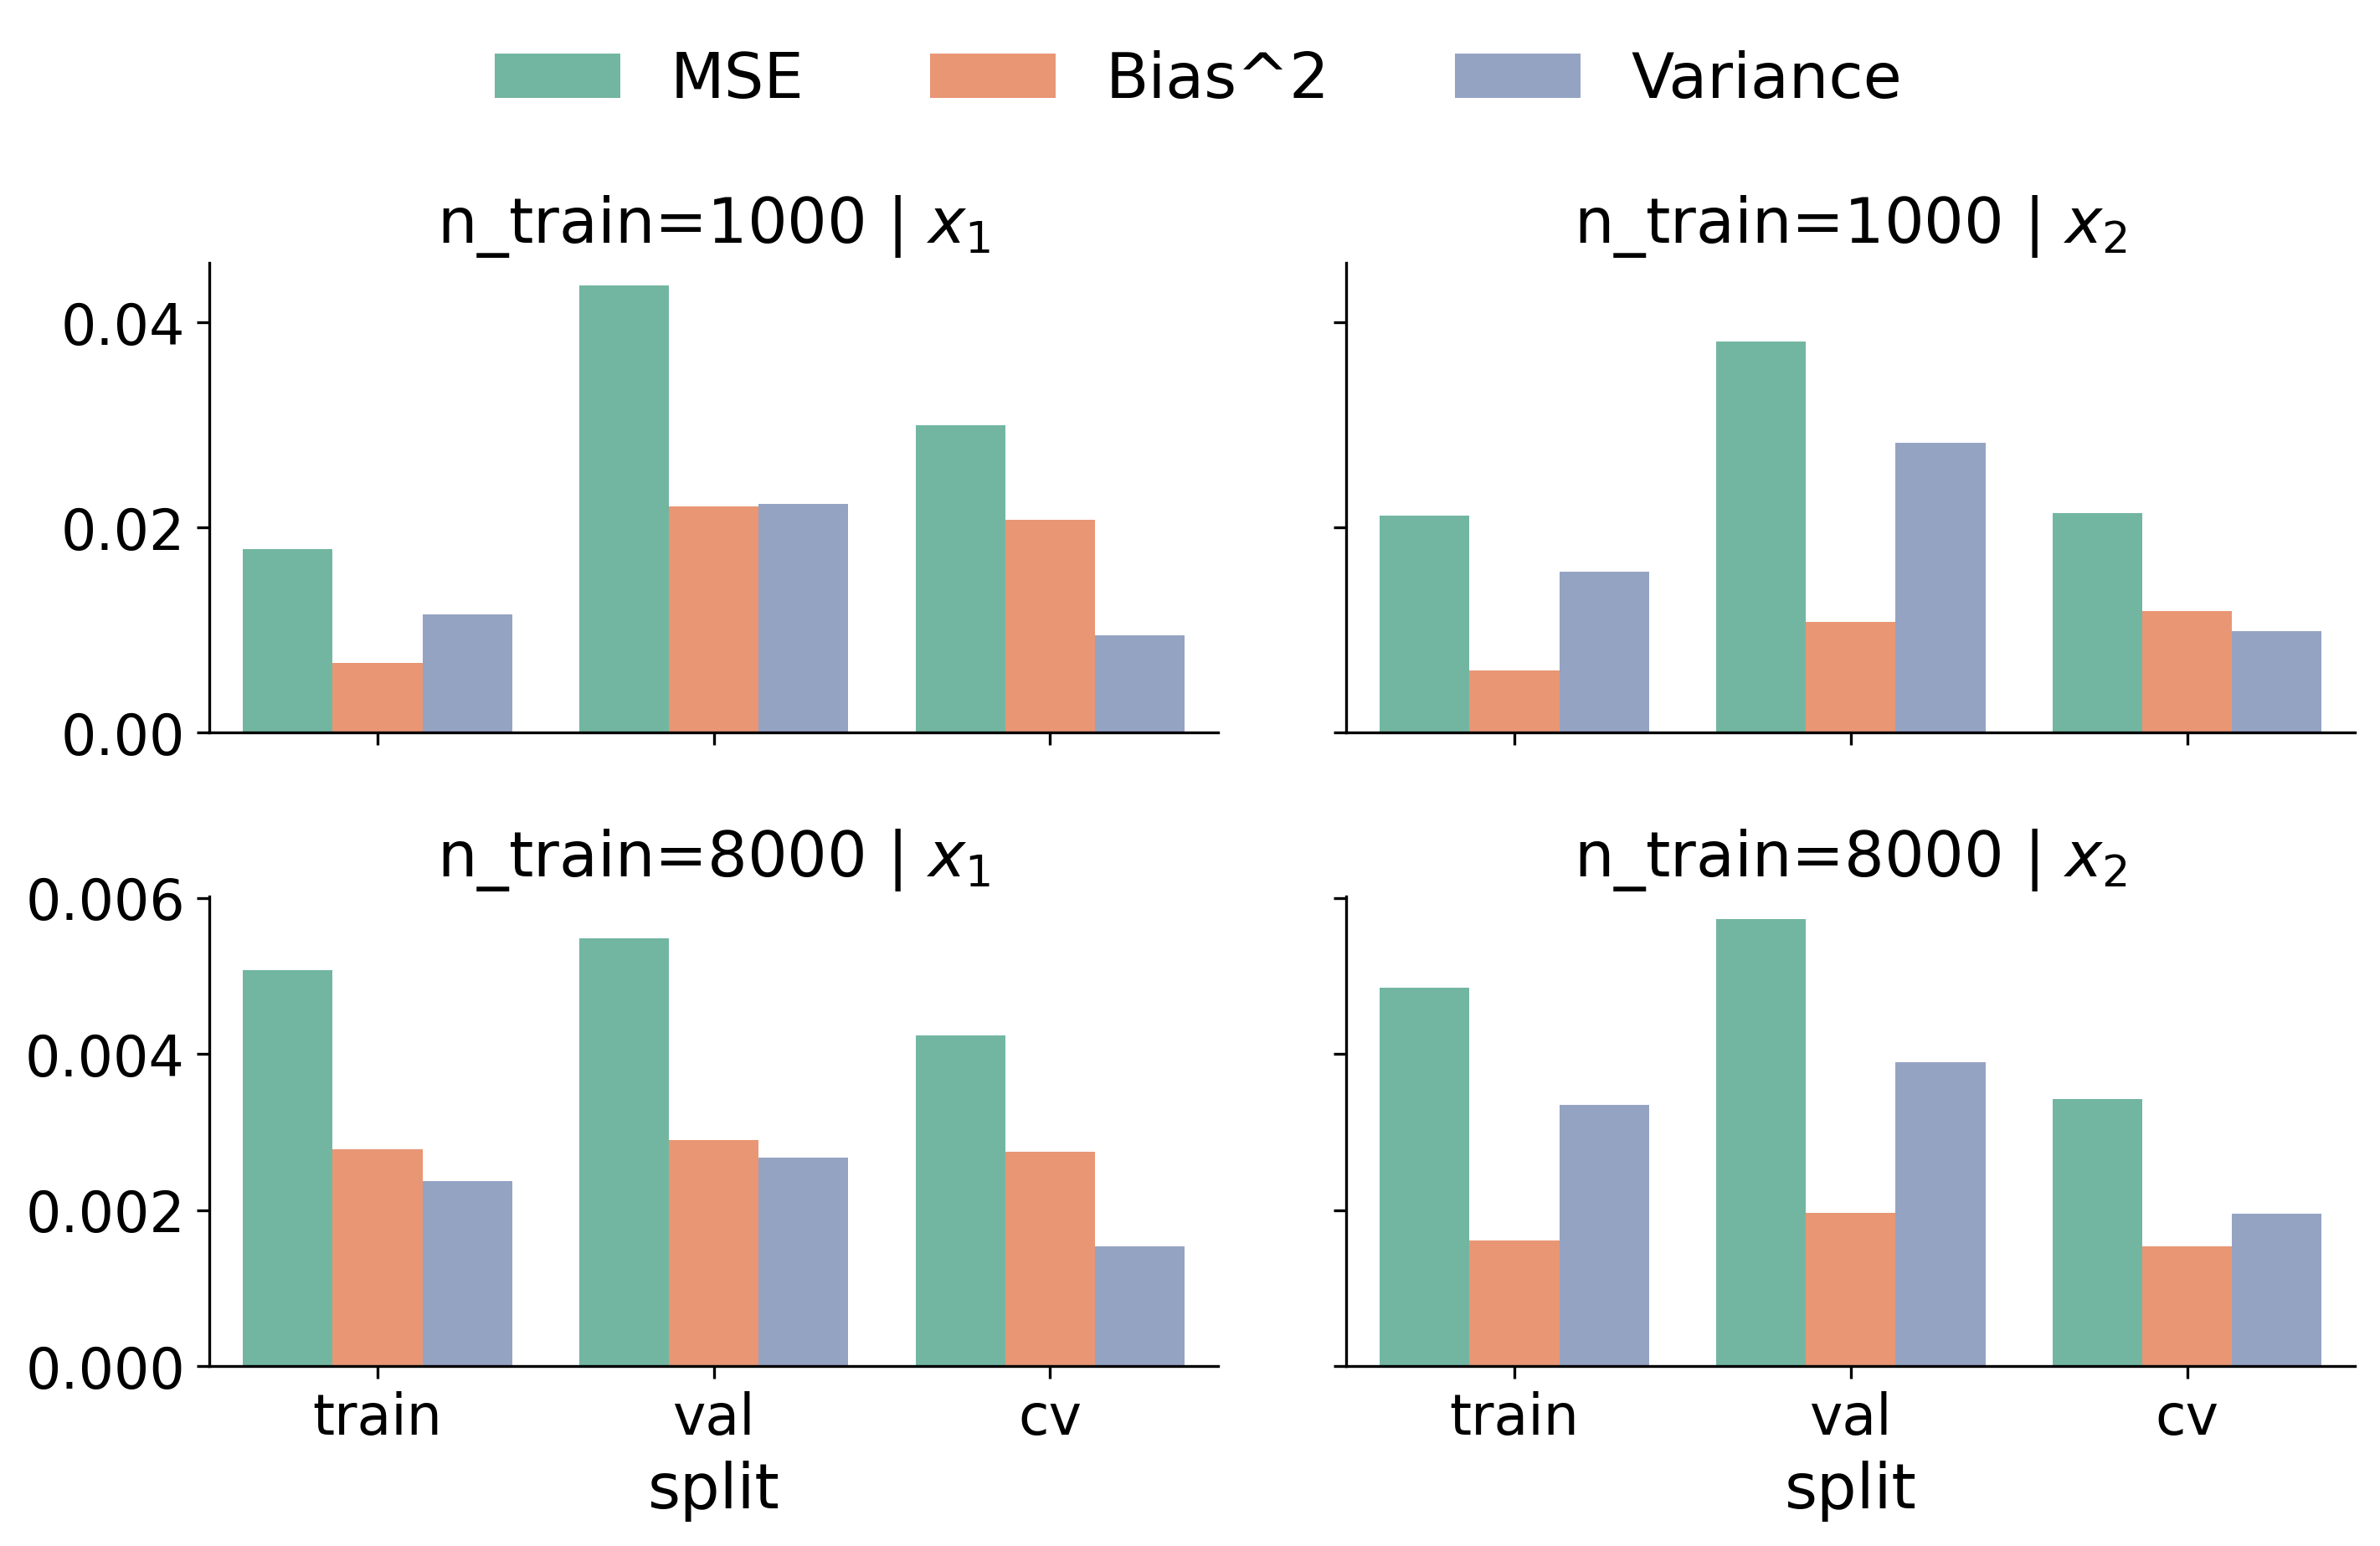
\includegraphics[width=\textwidth]{img/SNC/feature_effect_errors_ale_XGBoost_OT.png}
        \caption{XGBoost\_OT}
    \end{subfigure}
    \\[10pt]
    \vfill
    \begin{subfigure}[b]{0.49\textwidth}
        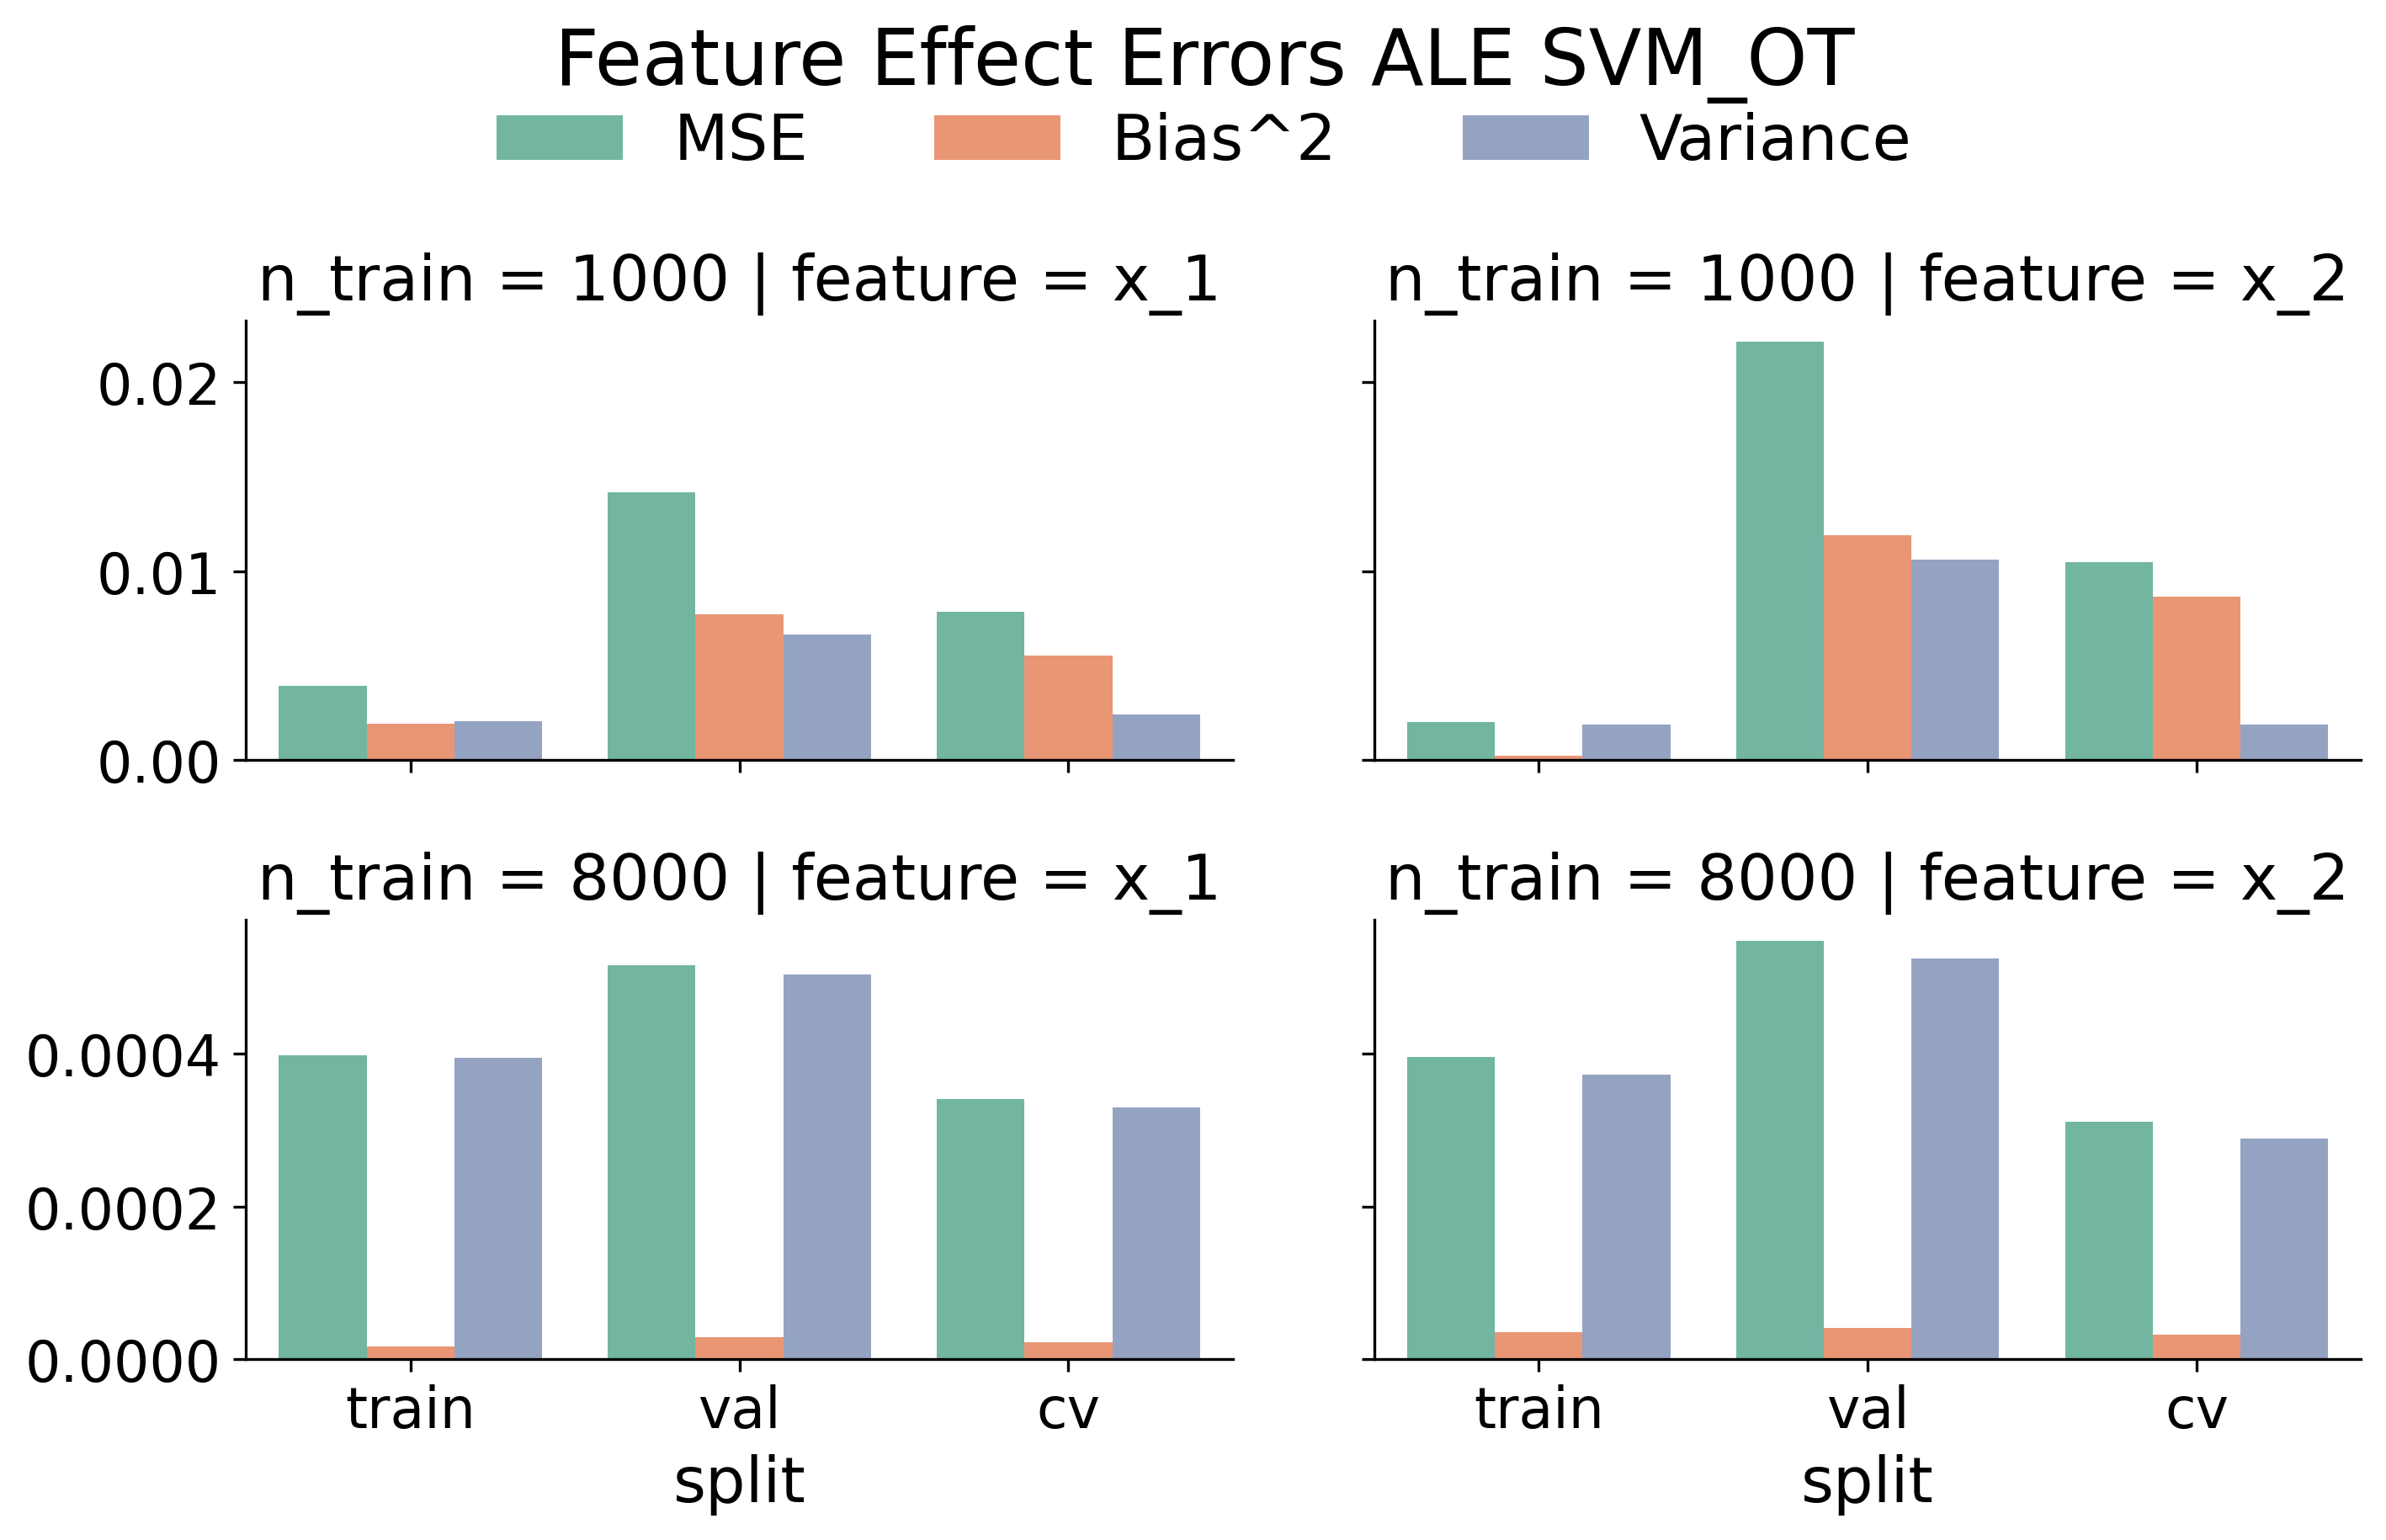
\includegraphics[width=\textwidth]{img/SNC/feature_effect_errors_ale_SVM_OT.png}
        \caption{SVM\_OT}
    \end{subfigure}
    \caption{Main experiment results for ALE on SimpleNormalCorrelated dataset. \dots}
    \label{fig:ale-results-snc}
 \end{figure}


\section{Conclusions}\label{sec:conclusion}

\subsection{Summary \& Discussion}

\subsection{Limitations \& Future Work}

\begin{credits}
    \subsubsection{\ackname} A bold run-in heading in small font size at the end of the paper is used for
    general acknowledgments, for example: This study was funded by X (grant number
    Y).

    \subsubsection{\discintname}
    The authors have no competing interests to declare that are relevant to the
    content of this article.
\end{credits}

%
% ---- Bibliography ----
\bibliographystyle{splncs04}
\bibliography{mybibliography}

% appendix
\newpage
\appendix
\section{Proof: Monte Carlo Variance for Groundtruth}\label{app:proof-mc-variance}
\begin{proof}
    For better readability, we will omit the subscript $S$ as well as the point $x_S$ and use $X=X_{mc}$ in this proof:

    \begin{align*}
        \mathbb{E}_F\mathbb{E}_X[(PDP_f - \widehat{PDP}_f)^2] & = \mathbb{E}_F\mathbb{E}_X[PDP_f^2 - 2PDP_f \widehat{PDP}_f + \widehat{PDP}_f^2]                                 \\
                                                              & = PDP_f^2 - 2PDP_f \mathbb{E}_F\mathbb{E}_X[\widehat{PDP}_f] + \mathbb{E}_F\mathbb{E}_X[\widehat{PDP}_f^2]       \\
                                                              & = PDP_f^2 - 2PDP_f^2 + \mathbb{E}_F\text{Var}_X[\widehat{PDP}_f] + \mathbb{E}_F[\mathbb{E}_X[\widehat{PDP}_f]^2] \\
                                                              & = PDP_f^2 - 2PDP_f^2 + \mathbb{E}_F\text{Var}_X[\widehat{PDP}_f] + PDP_f^2                                       \\
                                                              & = \mathbb{E}_F\text{Var}_X[\widehat{PDP}_f]                                                                      \\
                                                              & = \text{Var}_X[\widehat{PDP}_f]
    \end{align*}

    \noindent Again we use $\mathbb{E}_X[\widehat{PDP}_{f}] = PDP_{f}$ (cf.~\cite{molnar_relating_2023}) as well as the fact
    that all quantities based on $f$ do not depend on the model distribution $F$.
\end{proof}

\section{Model Hyperparameters and Performance}\label{app:model-hps-perf}
In this appendix, we give details on the models used in the simulation study.
Specifically, we provide details on the hyperparameter selection and the
finally used hyperparameters, as well as the performance of the models.

\subsection{Hyperparameters}

An overview of all hyperparameters used for the different models can be found
in \textbf{Table~\ref{tab:model-hyperparameters}}. Note that the linear
regression is excluded as we do not have any hyperparameters to tune.

Hyperparameters for the overfitting models (OF) were carefully hand-picked to
achieve strong performance on the training data while performing relatively
poorly on the validation data.

The optimal hyperparameters (OT) were chosen by tuning the models on a separate
data sample. Training and validation data were sampled independently from the
correspondings DGPs, with a training size of $n_{train}$ and a validation size
of 10000 to get a reliable performance estimate. While this scenario is
unrealistic in practice, it allows as to consider hyperparameters as
``pre-selected'' and avoid costly nested resampling strategies for the
simulation study. Each model was tuned for 200 trials using a
\textit{Tree-structured Parzen Estimator (TPE)}~\cite{bergstra2011algorithms}
using validation MSE as objective to minimize (equivalent to maximizing
R2-score).

\begin{table}
    \scriptsize
    \begin{tabularx}{\textwidth}{>{\RaggedRight\arraybackslash}m{1.6cm}p{1.225cm}p{2.05cm}>{\RaggedRight\arraybackslash}X}
        \toprule
        \textbf{Dataset}                        & \textbf{n\_train}                 & \textbf{Model}       & \textbf{Hyperparameters}                                                                                                                                                                          \\
        \midrule
        \multirow[t]{14}{=}{\textbf{Simple                                                                                                                                                                                                                                                                     \\Normal\\Correlated}} & \multirow[t]{7}{*}{\textbf{1000}} & \textbf{GAM\_OF} & n\_bases: 50; lam: 0.0005;  \\
        \textbf{}                               & \textbf{}                         & \textbf{GAM\_OT}     & n\_bases: 20; lam: 15.6807;                                                                                                                                                                       \\
        \textbf{}                               & \textbf{}                         & \textbf{SVM\_OF}     & C: 800; gamma: 10;                                                                                                                                                                                \\
        \textbf{}                               & \textbf{}                         & \textbf{SVM\_OT}     & C: 917.9061; gamma: 0.0030;                                                                                                                                                                       \\
        \textbf{}                               & \textbf{}                         & \textbf{XGBoost\_OF} & n\_estimators: 1200; max\_depth: 16; learning\_rate: 0.35; subsample: 1.0; min\_child\_weight: 1; colsample\_bytree: 1.0; colsample\_bylevel: 1.0; lambda: 0; alpha: 0;                           \\
        \textbf{}                               & \textbf{}                         & \textbf{XGBoost\_OT} & n\_estimators: 1640; max\_depth: 5; learning\_rate: 0.0062; subsample: 0.5601; min\_child\_weight: 1.6999; colsample\_bytree: 0.7632; colsample\_bylevel: 0.6944; lambda: 0.0156; alpha: 0.0660;  \\
        \cline{2-4}
        \textbf{}                               & \multirow[t]{7}{*}{\textbf{8000}} & \textbf{GAM\_OF}     & n\_bases: 64; lam: 1e-05;                                                                                                                                                                         \\
        \textbf{}                               & \textbf{}                         & \textbf{GAM\_OT}     & n\_bases: 5; lam: 0.0010;                                                                                                                                                                         \\
        \textbf{}                               & \textbf{}                         & \textbf{SVM\_OF}     & C: 1000; gamma: 10;                                                                                                                                                                               \\
        \textbf{}                               & \textbf{}                         & \textbf{SVM\_OT}     & C: 864.4724; gamma: 0.0085;                                                                                                                                                                       \\
        \textbf{}                               & \textbf{}                         & \textbf{XGBoost\_OF} & n\_estimators: 1500; max\_depth: 18; learning\_rate: 0.4000; subsample: 1.0; min\_child\_weight: 1; colsample\_bytree: 1.0; colsample\_bylevel: 1.0; lambda: 0; alpha: 0;                         \\
        \textbf{}                               & \textbf{}                         & \textbf{XGBoost\_OT} & n\_estimators: 2586; max\_depth: 5; learning\_rate: 0.0044; subsample: 0.9484; min\_child\_weight: 1.4257; colsample\_bytree: 0.8471; colsample\_bylevel: 0.8672; lambda: 5.1002; alpha: 0.0026;  \\
        \cline{1-4}
        \multirow[t]{14}{=}{\textbf{Friedman1}} & \multirow[t]{7}{*}{\textbf{1000}} & \textbf{GAM\_OF}     & n\_bases: 50; lam: 0.0001;                                                                                                                                                                        \\
        \textbf{}                               & \textbf{}                         & \textbf{GAM\_OT}     & n\_bases: 21; lam: 0.0402;                                                                                                                                                                        \\
        \textbf{}                               & \textbf{}                         & \textbf{SVM\_OF}     & C: 1000; gamma: 15;                                                                                                                                                                               \\
        \textbf{}                               & \textbf{}                         & \textbf{SVM\_OT}     & C: 917.1949; gamma: 0.2102;                                                                                                                                                                       \\
        \textbf{}                               & \textbf{}                         & \textbf{XGBoost\_OF} & n\_estimators: 1000; max\_depth: 14; learning\_rate: 0.3; subsample: 1.0; min\_child\_weight: 1; colsample\_bytree: 1.0; colsample\_bylevel: 1.0; lambda: 0; alpha: 0;                            \\
        \textbf{}                               & \textbf{}                         & \textbf{XGBoost\_OT} & n\_estimators: 2621; max\_depth: 8; learning\_rate: 0.0335; subsample: 0.6192; min\_child\_weight: 5.4066; colsample\_bytree: 0.7651; colsample\_bylevel: 0.5224; lambda: 11.6021; alpha: 4.5342; \\
        \cline{2-4}
        \textbf{}                               & \multirow[t]{7}{*}{\textbf{8000}} & \textbf{GAM\_OF}     & n\_bases: 80; lam: 1e-08;                                                                                                                                                                         \\
        \textbf{}                               & \textbf{}                         & \textbf{GAM\_OT}     & n\_bases: 22; lam: 0.0657;                                                                                                                                                                        \\
        \textbf{}                               & \textbf{}                         & \textbf{SVM\_OF}     & C: 1000; gamma: 18;                                                                                                                                                                               \\
        \textbf{}                               & \textbf{}                         & \textbf{SVM\_OT}     & C: 901.1903; gamma: 0.2602;                                                                                                                                                                       \\
        \textbf{}                               & \textbf{}                         & \textbf{XGBoost\_OF} & n\_estimators: 1200; max\_depth: 14; learning\_rate: 0.3; subsample: 1.0; min\_child\_weight: 1; colsample\_bytree: 1.0; colsample\_bylevel: 1.0; lambda: 0; alpha: 0;                            \\
        \textbf{}                               & \textbf{}                         & \textbf{XGBoost\_OT} & n\_estimators: 3691; max\_depth: 5; learning\_rate: 0.0070; subsample: 0.6643; min\_child\_weight: 1.4075; colsample\_bytree: 0.8403; colsample\_bylevel: 0.8186; lambda: 0.0399; alpha: 5.0734;  \\
        \cline{1-4}
        \multirow[t]{14}{=}{\textbf{Feynman                                                                                                                                                                                                                                                                    \\I.29.16}} & \multirow[t]{7}{*}{\textbf{1000}} & \textbf{GAM\_OF} & n\_bases: 50; lam: 0.0001;  \\
        \textbf{}                               & \textbf{}                         & \textbf{GAM\_OT}     & n\_bases: 31; lam: 0.3260;                                                                                                                                                                        \\
        \textbf{}                               & \textbf{}                         & \textbf{SVM\_OF}     & C: 200; gamma: 8;                                                                                                                                                                                 \\
        \textbf{}                               & \textbf{}                         & \textbf{SVM\_OT}     & C: 11.4317; gamma: 0.1394;                                                                                                                                                                        \\
        \textbf{}                               & \textbf{}                         & \textbf{XGBoost\_OF} & n\_estimators: 1000; max\_depth: 14; learning\_rate: 0.3; subsample: 1.0; min\_child\_weight: 1; colsample\_bytree: 1.0; colsample\_bylevel: 1.0; lambda: 0; alpha: 0;                            \\
        \textbf{}                               & \textbf{}                         & \textbf{XGBoost\_OT} & n\_estimators: 4246; max\_depth: 9; learning\_rate: 0.0327; subsample: 0.8004; min\_child\_weight: 6.3792; colsample\_bytree: 0.8420; colsample\_bylevel: 0.8357; lambda: 14.1131; alpha: 6.0556; \\
        \cline{2-4}
        \textbf{}                               & \multirow[t]{7}{*}{\textbf{8000}} & \textbf{GAM\_OF}     & n\_bases: 64; lam: 5e-07;                                                                                                                                                                         \\
        \textbf{}                               & \textbf{}                         & \textbf{GAM\_OT}     & n\_bases: 32; lam: 0.4500;                                                                                                                                                                        \\
        \textbf{}                               & \textbf{}                         & \textbf{SVM\_OF}     & C: 400; gamma: 10;                                                                                                                                                                                \\
        \textbf{}                               & \textbf{}                         & \textbf{SVM\_OT}     & C: 22.5167; gamma: 0.1114;                                                                                                                                                                        \\
        \textbf{}                               & \textbf{}                         & \textbf{XGBoost\_OF} & n\_estimators: 1000; max\_depth: 14; learning\_rate: 0.3; subsample: 1.0; min\_child\_weight: 1; colsample\_bytree: 1.0; colsample\_bylevel: 1.0; lambda: 0; alpha: 0;                            \\
        \textbf{}                               & \textbf{}                         & \textbf{XGBoost\_OT} & n\_estimators: 3962; max\_depth: 7; learning\_rate: 0.0372; subsample: 0.9351; min\_child\_weight: 4.0962; colsample\_bytree: 0.8640; colsample\_bylevel: 0.7728; lambda: 29.2036; alpha: 5.1631; \\
        \bottomrule
    \end{tabularx}
    \caption{Hyperparameters for the models used in the simulation study}
    \label{tab:model-hyperparameters}
\end{table}

\subsection{Model Performance Evaluation}

To ensure that the models perform as expected, we evaluate their performance
both on the training data and a holdout test data with the latter consisting of
10000 samples to get a reliable performance estimate. The performances
evaluated over the 30 repetitions are aggregated in
\textbf{Fig.~\ref{fig:model-performance}} showing the R2-scores. As intended,
the overfitting models perform better on the training data than the optimally
tuned models, while being outperformed on the holdout test data and also
exhibiting higher variance in their generalization performance. Note that the
linear regression model serves only as a baseline. The overfitted SVM (SVM\_OF)
show substantially worse performances on test data compared to the other
models. Therefore, we excluded it from further analysis.

\begin{figure}
    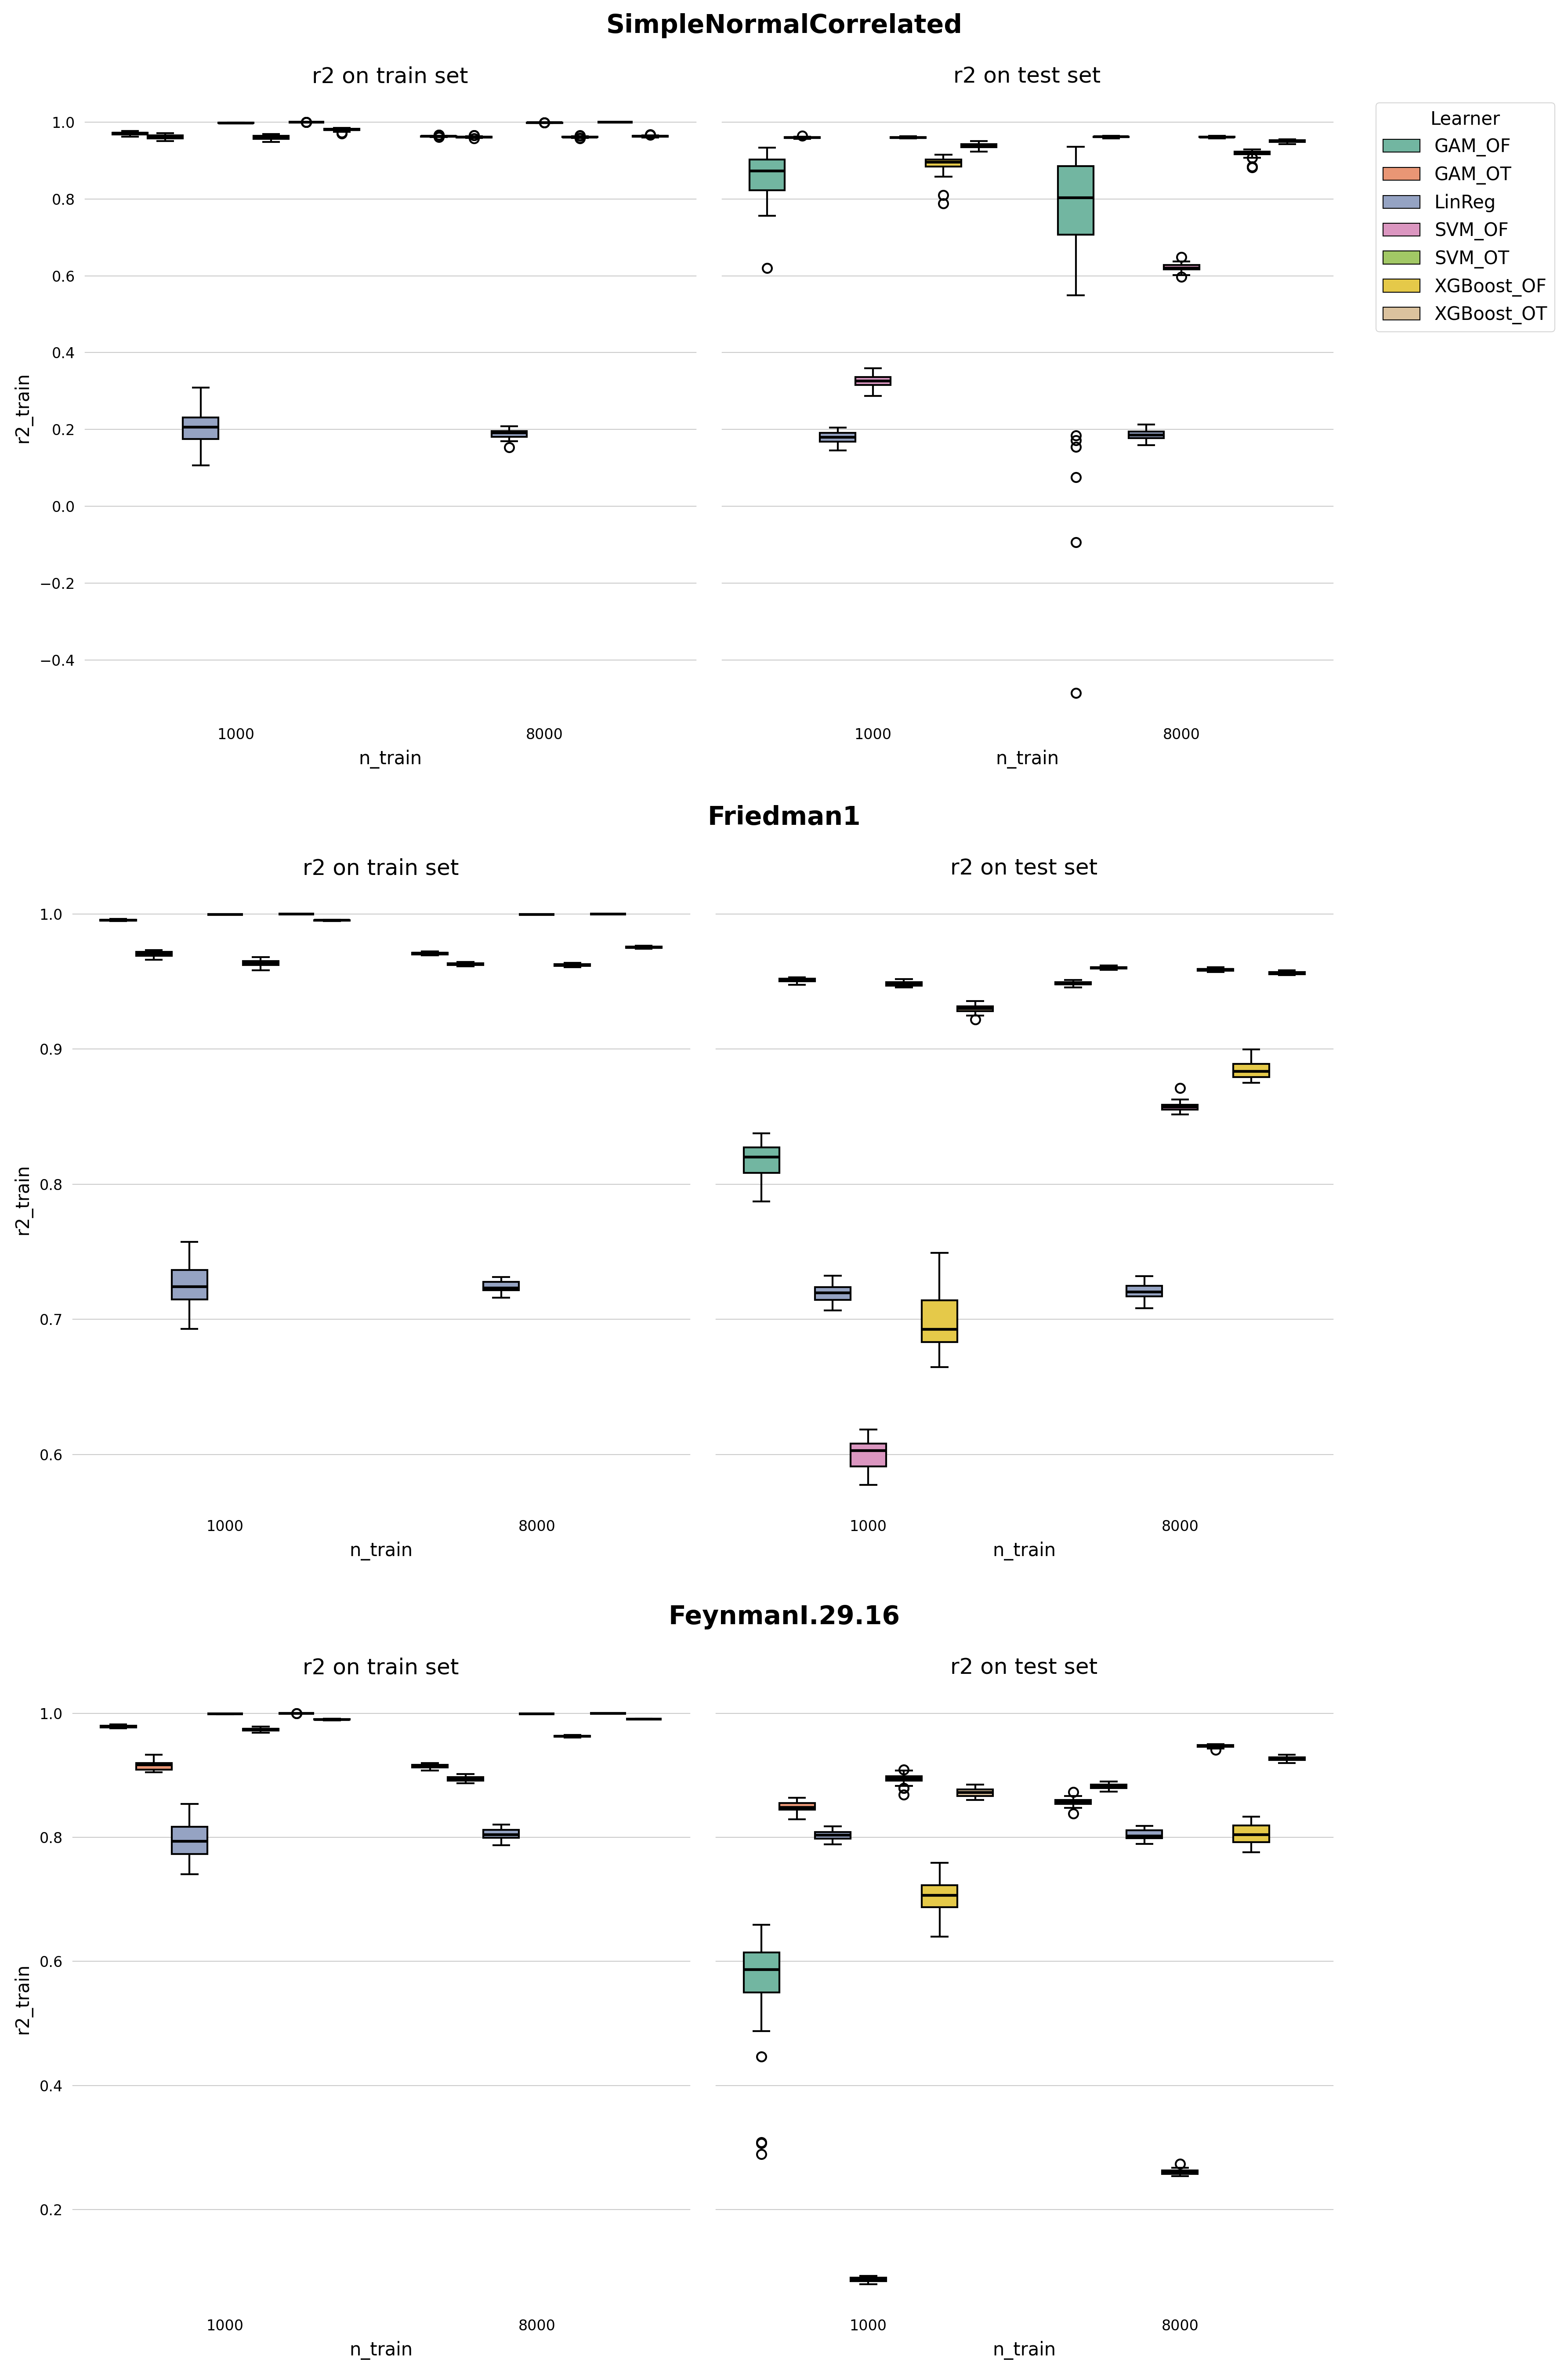
\includegraphics[width=\textwidth]{img/model_performances.png}
    \caption{R2-score of the models on training (left) and holdout test data (right), each boxplot aggregates 30 repetitions}
    \label{fig:model-performance}
\end{figure}

\end{document}
